\chapter{Results and discussion}\label{chap:Results&Disc}
In this chapter the results from laboratory experiments are presented and discussed.

\section{PFCA sorption behavior}
\subsection{Biochar-water sorption isotherms}
\cref{fig:sorption_isotherms} shows the sorption isotherms for PFPeA, PFHxA, PFHpA, PFOA, PFNA and PFDA on CWC, ULS and DSL. The points generated from the batch tests were fitted using the Freundlich model (\cref{eq:FreundlichLinear}). For all compounds, the sorption isotherm for ULS is visibly higher than DSL, followed by CWC. The Freundlich sorption coefficients ($log~K_F$), linearity coefficients ($n_F$) and correlation coefficients ($r^2$) are presented in \cref{tab:summary_stats_single}. Somewhat unexpectedly, sorption is strongest for the two sludge chars. Possible mechanisms for the strong sorption will be discussed in this section. 

Due to the novel research on sewage sludge biochars as sorbents for PFAS in this thesis, literature partitioning coefficients for PFCAs to other sewage sludge biochars are non-existent to the author's knowledge. However, comparisons can be made between the $log~K_F$s found in this thesis and for commercially-produced activated carbons (AC) reported in other studies, which  The sorption coefficients are equivalent or higher compared to literature values for $log~K_F$ of PFOA to AC: 5.60 \citep{Kupryianchyk2016a}, 4.45 \citep{hansen2010sorption}, and 4.74-5.42 \citep{silvani2019can}.

\begin{figure}[tb]
    \centering
    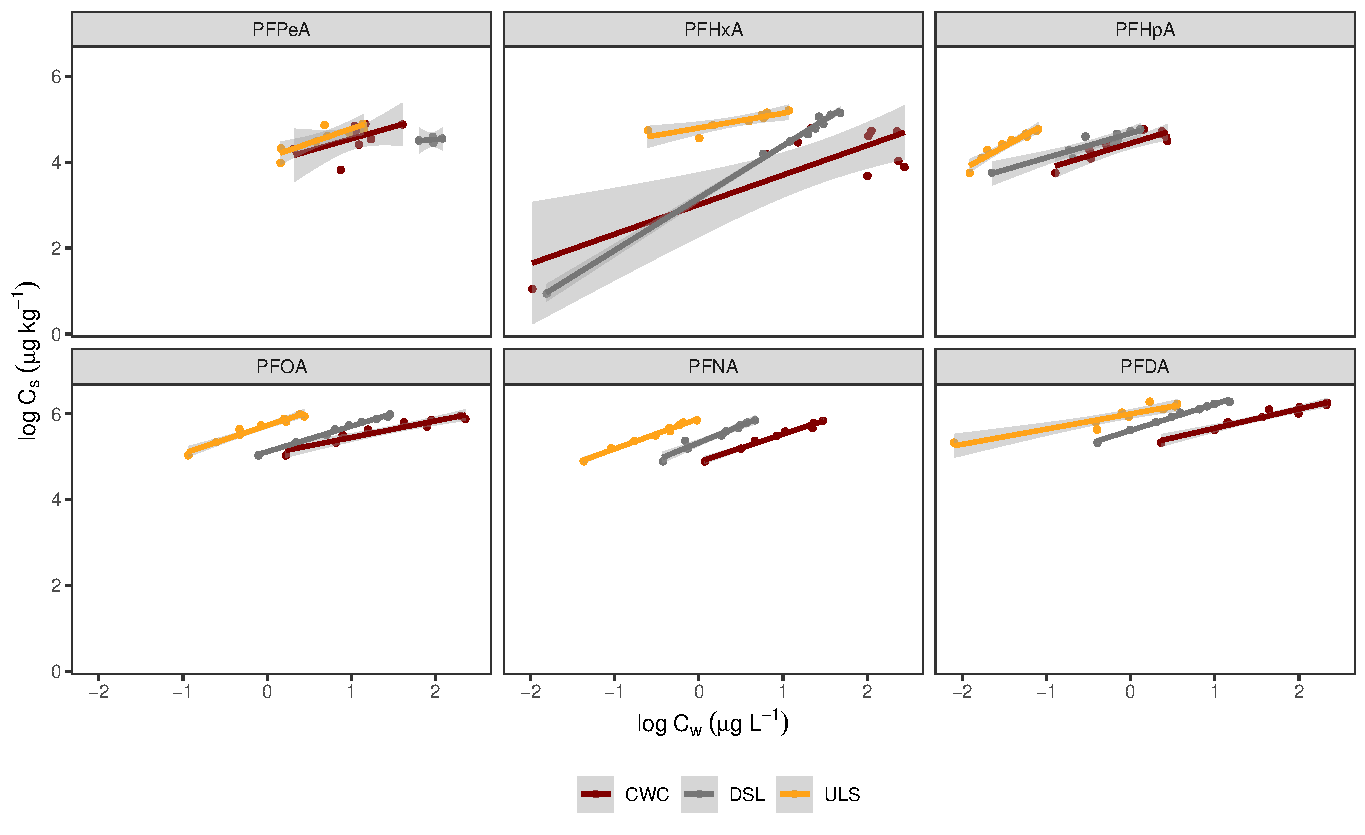
\includegraphics[width=0.8\textwidth]{R/figs/Sorption_isotherms_single_BC.pdf}
    \caption{Freundlich sorption isotherms of TCs in batch tests with three different biochars. Lines are obtained by linear regression.}
    \label{fig:sorption_isotherms}
\end{figure}

\begin{figure}[tb]
    \centering
    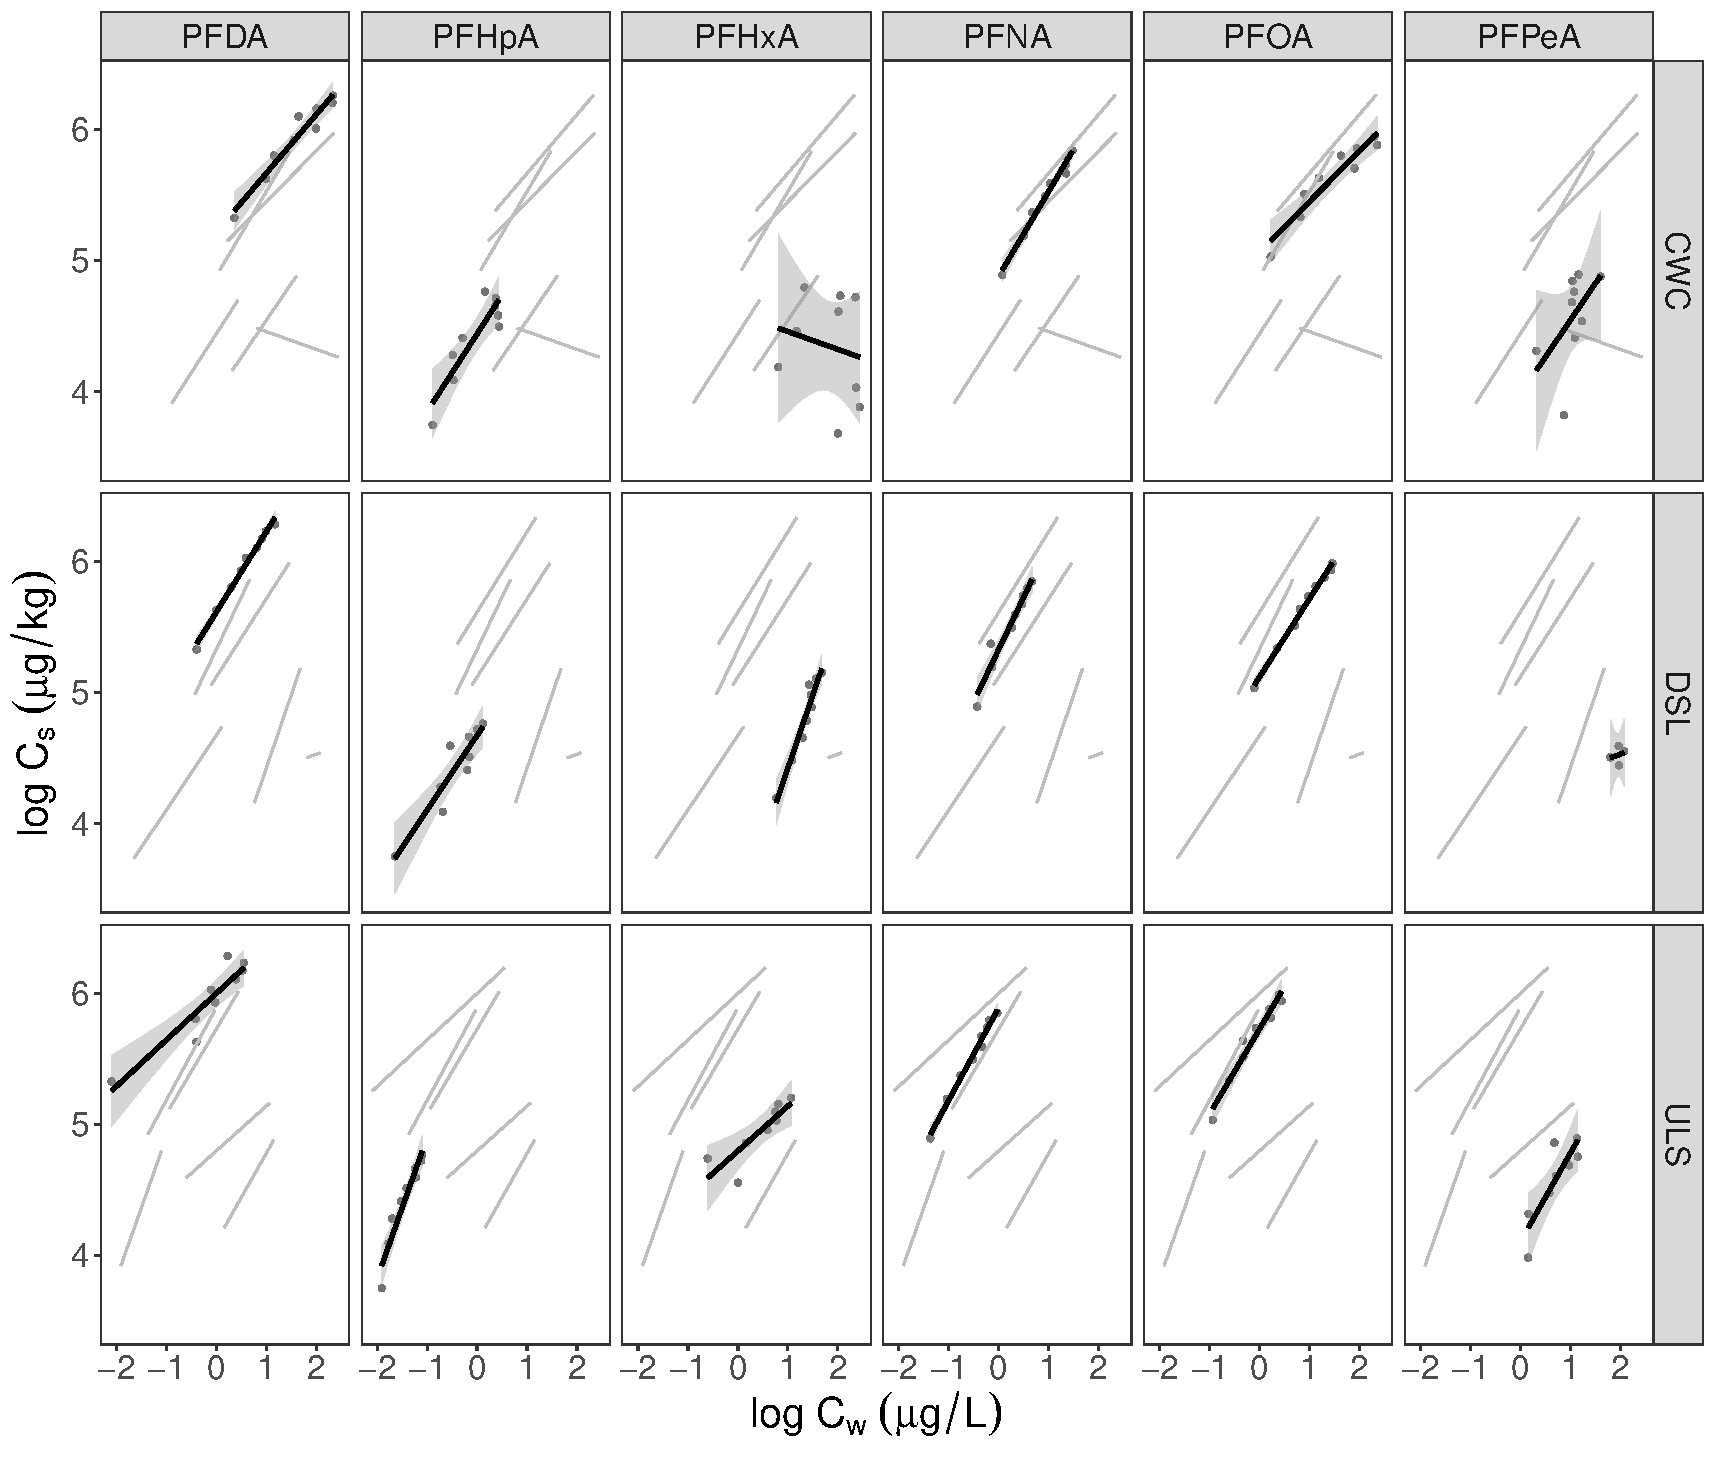
\includegraphics[width=\textwidth]{R/figs/BC_facet_isotherm.pdf}
    \caption{Single-compound Freundlich sorption isotherms of PFPeA, PFHxA, PFHpA, PFOA, PFNA and PFDA. Lines are obtained by linear regression. For comparison across chain length, the shaded gray lines are the isotherms from the other compounds with the same sorbent.}
    \label{fig:sorption_isotherms_all}
\end{figure}

\begin{table}
\caption{Freundlich sorption parameters of single TC isotherms in CWC, ULS and DSL (n=9). The error is presented as standard error. All $K_F$ data are in units of $\mathrm{(\mu g/kg)/(\mu g/L)^{n_F}}$.}
\centering
\adjustbox{max width=\textwidth}{%
\begin{threeparttable}
\label{tab:summary_stats_single}
\begin{tabular}{lllllllllllll} \toprule
PFCA & \multicolumn{4}{c}{ULS} & \multicolumn{4}{c}{DSL} & \multicolumn{4}{c}{CWC} \\ \cmidrule(l){2-5} \cmidrule(l){6-9} \cmidrule(l){10-13}
 & $log~K_{F,BC}$ & $n_{F,BC}$ & $r^2$ & $p$ & $log~K_{F,BC}$ & $n_{F,BC}$ & $r^2$ & $p$ & $log~K_{F,BC}$ & $n_{F,BC}$ & $r^2$ & $p$ \\ \midrule
PFPeA & 4.10 ± 0.13 & 0.67 ± 0.16 & 0.74 & ** & 4.25 ± 0.74 & 0.14 ± 0.38 & 0.06 & $>$0.05 & 3.98 ± 0.36 & 0.56 ± 0.33 & 0.30 & $>$0.05 \\
PFHxA & 4.80 ± 0.06 & 0.34 ± 0.09 & 0.72 & ** & 3.30 ± 0.15 & 1.11 ± 0.11 & 0.93 & *** & 4.59 ± 0.50 & -0.14 ± 0.26 & 0.04 & $>$0.05 \\
PFHpA & 5.98 ± 0.17 & 1.08 ± 0.11 & 0.93 & *** & 4.67 ± 0.06 & 0.57 ± 0.09 & 0.86 & *** & 4.44 ± 0.05 & 0.59 ± 0.11 & 0.80 & ** \\
PFOA & 5.73 ± 0.02 & 0.65 ± 0.05 & 0.95 & *** & 5.12 ± 0.02 & 0.60 ± 0.02 & 0.99 & *** & 5.06 ± 0.08 & 0.39 ± 0.05 & 0.90 & *** \\
PFNA & 5.89 ± 0.02 & 0.71 ± 0.03 & 0.99 & *** & 5.33 ± 0.03 & 0.80 ± 0.07 & 0.94 & *** & 4.88 ± 0.04 & 0.65 ± 0.04 & 0.98 & *** \\
PFDA & 6.00 ± 0.04 & 0.35 ± 0.05 & 0.86 & *** & 5.61 ± 0.02 & 0.61 ± 0.02 & 0.99 & *** & 5.22 ± 0.07 & 0.45 ± 0.04 & 0.94 & *** \\ \bottomrule
\end{tabular}
\begin{tablenotes}
\item Significant codes: *** $\sim$ 0.001, ** $\sim$ 0.01  
\end{tablenotes}
\end{threeparttable}}
\end{table}

\subsection{Effect of PFCA properties}
\subsubsection{PFCA chain length}
\cref{fig:sorption_isotherms_all} shows sorption isotherms for the single-compound batch tests for CWC, ULS and DSL. The Freundlich coefficients ($log~K_F$) for ULS increased in the order: PFPeA (CF4) $<$ PFHxA (CF5) $<$ PFOA (CF7) $<$ PFHpA (CF6) $<$ PFNA (CF8) $<$ PFDA (CF9), ranging from 4.10$\pm$0.13 to 6.00$\pm$0.04, all regressions being significant (p$<$0.01), \cref{tab:summary_stats_single}). The Freundlich coefficients for DSL increased in the order, PFHxA (CF5) $<$ PFPeA (CF4) $<$ PFHpA (CF6) $<$ PFOA (CF7) $<$ PFNA (CF8) $<$ PFDA (CF9), ranging from $log~K_F$ 3.30$\pm$0.15 to 5.61$\pm$0.02. All regressions were significant (p$<$0.001) except for the PFPeA isotherm which only consisted of four points (SP7-10) because several points that had a higher analyzed filtrate concentrations than what was spiked for SP1-6 had to be omitted (analytical uncertainty or imprecision/contamination during laboratory work) (\cref{fig:sorption_isotherms_all}). The Freundlich coefficients for CWC increased in the order, PFPeA (CF4) $<$ PFHpA (CF6) $<$ PFHxA (CF5) $<$ PFNA (CF8) $<$ PFOA (CF7) $<$ PFDA (CF9), ranging from $log~K_F$ 3.98$\pm$0.36 to 5.22$\pm$0.07. Regressions were significant (p$<$0.01) except for PFPeA and PFHxA. 

A statistically significant relationship between $log~K_F$ and CF\textsubscript{2} chain length was found for all three biochars (p$<$0.05) \cref{fig:chainlength}, which is in accordance with previous studies \citep{Sorengard2019, higgins2006sorption, ahmed2020per}. There was a difference of 1.2-1.9 $log~K_F$ units between the longest and the shortest PFCA chain (PFDA and PFPeA). For every CF\textsubscript{2} moiety, hydrophobic interactions between condensed aromatic structures in the biochar matrix increases, contributing to stronger sorption. Several mechanisms can be used to explain why perfluorinated carboxylic acids increase in hydrophobicity with increasing chain length: 1) due to high molecular surface of the perfluorinated tail, a high cavity formation energy is needed to dissolve the compounds in water, and therefore they tend to be pushed towards water extremities, such as a biochar surface. Therefore, dissolution becomes increasingly energetically demanding with increasing chain length \citep{sigmund2022sorption}. 2) the perfluorinated chain with CF\textsubscript{2} moieties is capable of the least van der Waals interactions per molecular surface area compared to CH\textsubscript{2} which results in the least interactions between water molecules when in the water cavity. This is why PFASs are both oil- and water repellent.  Generally, these forces have shown to be insignificant for sorption of PFAS to solid phases for short-chain molecules (\textless C6) but is significant for long-chained PFCs (\textgreater C6) \citep{du2014adsorption}.
London dispersion forces (induced dipole-induced dipole attraction), the weakest intermolecular force make the bonding so strong, not Van der Waals forces,  separation distance, condensed aromatic carbon surfaces \citep{Cornelissen2005}

\begin{figure}[tbh]
    \centering
    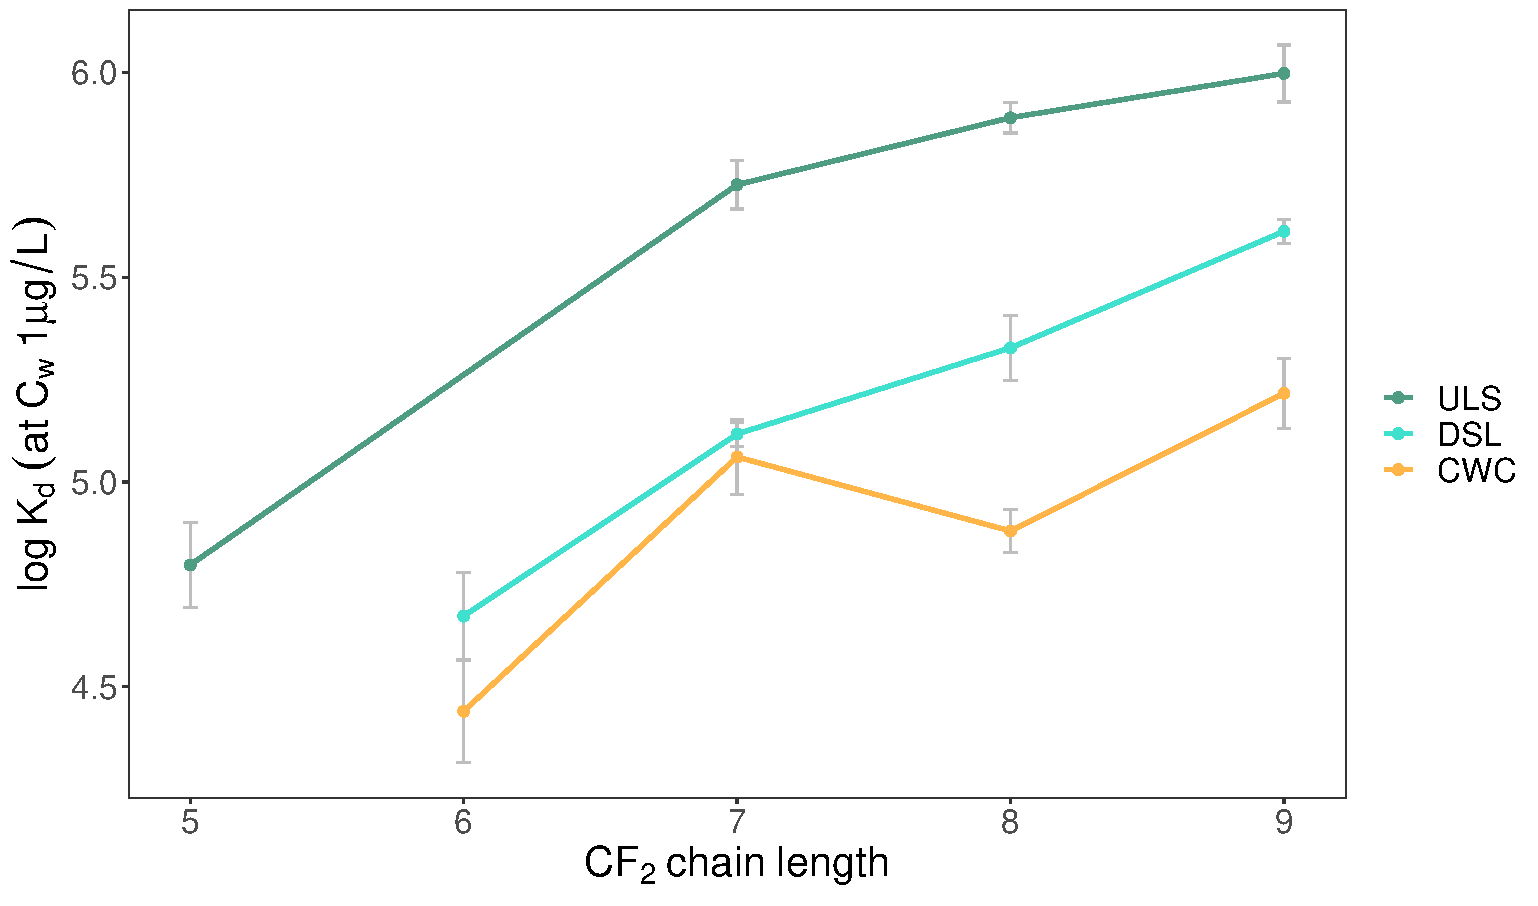
\includegraphics[width=0.7\textwidth]{R/figs/chain_length_Kd1ugL_plot.pdf}
    \caption{Relationship between $log~K_F$ and chain length. Linear regression coefficients for ULS: $r^2$ = 0.92, $p$ = 0.04, DSL: $r^2$ = 0.98, $p$ = 0.01, CWC: $r^2$ = 0.68, $p$ = 0.17. Error bars are the propagated error of $log~K_F$ and $n_F$.}
    \label{fig:chainlength}
\end{figure}

\subsubsection{PFAS functional group} 
\cite{zhang2021sorption} found that sorption increased in the order PFBA $<$ PFBS $<$ PFOA $<$ PFOS for granular activated carbon and softwood-derived biochar. The difference between the PFSA and PFCA groups is that PFSAs have one more perfluorinated carbon than PFCAs, which has its terminal carbon bonded as a carboxylate (COO\textsuperscript{-}). If one compares PFHpS with PFOA, which have the same number of $\mathrm{CF_2}$ moieties, the perfluorinated sulfonic acid still sorbs better. Researchers attribute this to 1) difference in molecular size, where the sulfonate moiety is slightly larger than the carboxylate moiety, which results in greater cavity formation energy of PFSAs, and hence in water saturated conditions, the functional group is pushed towards water extremities \citep{yin2022insights,sigmund2022sorption}. In batch shaking experiments this would be the biochar surfaces or tube walls; 2) Because sulfonic acid is a stronger acid than carboxylic acid which results in stronger ionic interaction to positive charges of mineral phases \citep{arvaniti2015review}. \cite{du2014adsorption}: electr and hydry balance The results for PFPeA, PFHxA and PFHpA are more sporadic and lower sorption, which can be indicative of hydrophobic interaction being the dominant mechanism of sorption and that electrostatic attractions occur more sporadic.Since sorption increased with chain length onto all three biochars in this study, this suggests that hydrophobic interactions is the dominant sorption mechanism over electrostatic interactions. Therefore, further investigation to explain why the sludge biochars sorb better than CWC is described in the next section. 

The charged and polar head of PFCAs give these compound classes unique sorptive properties because the polar head can engage simultaneously in electrostatic bonding with surface functional groups or bridging cations within the biochar matrix (ash rich in cations) \citep{zhang2013sorption,sigmund2022sorption}. In this study, the highest sorption were seen for ULS and DSL with the lowest \% C (\cref{tab:SAPV}), which is, at large, in contrast with previous literature. However, previous PFAS sorption studies have been conducted on biochar from cleaner, wood-based feedstock \citep{Sormo2021}, activated carbon \citep{zhang2021sorption,Kupryianchyk2016b}, soils and sediments \citep{higgins2006sorption}, and raw sewage sludges \citep{zhang2013sorption}. These studies conclude that the importance of electrostatic interaction to sorption comes secondary to the hydrophobic effect. The main reason for this is that the biochar surface is net negatively charged with a high cation exchange capacity (CEC) \citep{Ahmad2014} and may experience electrostatic repulsion of the negatively charged functional group on the PFAS (Include PZC when available). PFCAs have low $pK_a$s (-1, \citep{goss2008pKa}) due to having strong electron withdrawing fluorine atoms and hence become strong acids. The PFCAs investigated in this study will be negatively charged given the filtrate pH of 7.1-7.4 (\cref{tab:pHcond}). Thus, all target compounds experience electrostatic repulsion from the biochar surface which result in the lowest $K_F$-values for the shorter-chain PFCAs (\cref{tab:summary_stats_single}). Electrostatic repulsion is reduced in acid soils where the CEC is reduced and the biochar surfaces become protonated and more neutral. This allows for anion- \textpi-bond interaction with biochar \citep{sigmund2022sorption}. 

%%%%%%%%%%%%%%%%%%%%%%%%%%%%%%%%%%%%%%%%%%%%%%%%%%%%%%%%%%%%%%%%%%%%%%%%%%%%%%%%%%%%%%%%%%%%%%%%%%%%%%%%%%%%%%%%%%%%%%%%%%%%%%%%%%%%%%%%%%%%%%%%%%%%%%%%%%%%%%%%%%%%%%%%%%%%%%%%%%%%%%%%%%%%%%%%%%%%%%%%%%%%%%%%%%%%%%%%%%%%%%%%%%%%%%%%%%%%%%%%%%%%%%%%%%%%%%%%%%%%%%%%%%%%%%%%%%%%%%%%%%%%%%%%%%%%%%%%%%%%%%%%%%%%%%%%%%%%%%%%%%%%%%%%%%%%%%%%%%%%%%%%%%%%%%%%%%%%%%%%%%%%%%%%%%%%%%%%%%%%%%%%%%%%%%%%%%%%%%%%%%%%%%%%%%%%%%%%%%%%%%%%%%%%%%%%%%%%%%%%%%%%%%%%%%%%%%%%%%%%%%%%%%%%%%%%%%%%%%%%%%%%%%%%%%%%%%%%%%%%%%%%%%%%%%%%%%%%%%%%%%%%%%%%%%%%%%%%%%%%%%%%

\section{Effect of biochar properties on sorption}
This section compares the distribution coefficients derived for ULS, DSL and CWC to biochar composition of main elements (C, H, O, N), trace elements (Ca and Fe), surface area (SA) and pore volume (PV) in order to gain insights into possible sorption mechanisms. In the comparison between sorbent properties and sorption coefficients for each biochar feedstock, PFOA, PFNA and PFDA have been used because they gave the best sorption isotherms. $log~K_F$ has been normalized to 1 $\mu g~L^{-1}$ which is used as the distribution coefficients in this discussion.

\subsection{Surface area and pore volume}

\begin{table}
\centering
\caption{Surface area (SA), pore volume (PV), elemental content (C, O, H, N) and ratios for the biochars produced for the batch tests.}
\adjustbox{max width=\textwidth}{
\label{tab:SAPV}
\begin{tabular}{llrrrrrrlllllll}
\toprule
Biochar & Pyrolysis & \multicolumn{3}{l}{N\textsubscript{2} sorption} & \multicolumn{3}{l}{CO\textsubscript{2} sorption} & \multicolumn{4}{c}{Elemental content} & \multicolumn{3}{c}{Elemental ratio} \\
sorbent & temperature & \multicolumn{3}{l}{(pores \textgreater 1.5 nm)} & \multicolumn{3}{l}{(pores 0.4-1.5 nm)} & & & & & & & \\ \cmidrule(l){3-5} \cmidrule(l){6-8} \cmidrule(l){9-12} \cmidrule(l){13-15} & (\textdegree C) & BET SA  & BJH PV & log SA/PV & DFT SA & DFT PV & log SA/PV & C & O & H & N & O/C & H/C & N/C \\
& & ($\mathrm{m^2~g^{-1}}$) & (cm\textsuperscript{3} g\textsuperscript{-1}) & ($\mathrm{m^2 cm^{-3}}$) & ($\mathrm{m^2~g^{-1}}$) & (cm\textsuperscript{3} g\textsuperscript{-1}) & ($\mathrm{m^2 cm^{-3}}$) & (\%) & (\%) & (\%) & (\%) & & & \\ \midrule
CWC & 700 & 323 & 0.017 & 3.21 & 683 & 0.186 & 3.54 & 91.4 & 5.50 & 1.01 & 0.69 & 0.06 & 0.01 & 0.008       \\
ULS & 700 & 128 & 0.126 & 2.80 & 165 & 0.047 & 3.57 & 29.6 & 57.1 & 1.24 & 1.13 & 1.9  & 0.04 & 0.04        \\
DSL & 700 & 110 & 0.111 & 2.80 & 87  & 0.027 & 3.51 & 13.5 & 61.4 & 1.05 & 0.82 & 4.6  & 0.08 & 0.06       \\ \bottomrule
\end{tabular}}
\end{table}

\subsubsection{Pore size distribution between 0.4-1.5 nm}
\cref{tab:SAPV} shows the total surface area (SA, m\textsuperscript{2}/g) and pore volume (PV, cm\textsuperscript{3}/g) for the three biochars used in the sorption experiments in this study. SA of CWC was $\sim$six times higher than ULS and DSL (165 and 87  m\textsuperscript{2} g\textsuperscript{-1}, respectively), and PV also followed the same order. Previous research have postulated that large internal surface area and pore volume are desirable for strong sorption of organic contaminants because it increases the fraction of active sorption sites \citep{ahmed2020per,Hale2016}. The high SA and PV of CWC suggests that this biochar has the highest fraction of active sites compared to ULS and DSL within the micropore range ($\le$ 2 nm). However, pore size distribution (PSD) in terms of SA and PV of pores available for CO\textsubscript{2} adsorption (0.4-1.5 nm) is shown in \cref{fig:PZD_small}, where it becomes becomes evident that nearly 80\% of the SA and 60\% of the PV of CWC is located pores smaller than 0.6 nm, referred to as ultra micropores \citep{bardestani2019experimental}. \cref{tab:molecsize} lists effective cross-sectional diameter ($D_{eff}$) and maximum diameter ($D_{max}$) of each TC (the definitions of $D_{eff}$ and $D_{max}$ are illustrated in \cref{fig:molecularSize}). PFCAs C5-C10 range from 0.45-0.72 nm $D_{eff}$ and 0.96-1.54 nm $D_{max}$. Since the respective perfluorinated chains are too large and rigid to enter, most pores within the CO\textsubscript{2} fraction are nearly inaccessible to the adsorbate molecules \citep{yu2009sorption}. Additionally, too small pores makes it difficult for the compounds to adapt their shape to the pore wall to be able to come close enough to sorb to the surface and may for this reason get stuck in a cross-sectional position that blocks the pores for diffusion of new sorbates. 

The surface area to pore volume ratio can be used to more accurately represent available sorption sites where a lower ratio is indicative of higher porosity \citep{presser2011SAPV}. Since PV increases by increasing pore diameter (\cref{fig:PZD_small}), the relative increase in PV will be higher than the relative increase in SA, which means that the SA/PV ratio is expected to decrease more rapidly for biochar with higher pore volumes. This expectation is confirmed in \cref{fig:PZD_small} where the SA/PV ratios for ULS and DSL are nearly equivalent to CWC despite SA and PV being significantly different from CWC taken separately. This is reflected in the cumulative SA/PV ratios (\cref{tab:SAPV}) which are similar: 3 674, 3 502, and 3 206 m\textsuperscript{2} cm\textsuperscript{-3} for CWC, ULS, and DSL respectively. This means that despite CWC being far more numerous in micropores than ULS and DSL, the porosity of these pores are similar and is predominantly allocated within the ultra micropore fraction.

Maximum sorption is acheived when the molecular dimensions of PFAS match the pore size and shape of the sorbent \citep{Hale2016}. Since the PSD within the CO\textsubscript{2}-range is dominated by pores ultra micropores, sorption of PFPeA, PFHxA, and PFHpA is only possible if the congeners enter the pores at the exact right angle. PFOA, PFNA, and PFDA will experience size exclusion because the molecular size is too large in any direction (\cref{tab:molecsize}). Additionally, these pores are easily blocked. Therefore, sorption of PFAS in the CO\textsubscript{2}-range is insignificant and cannot explain the differences in $log~K_F$ between biochar feedstocks, especially since strongest sorption was measured for long-chain PFCAs.

\begin{figure}[htb]
    \centering
    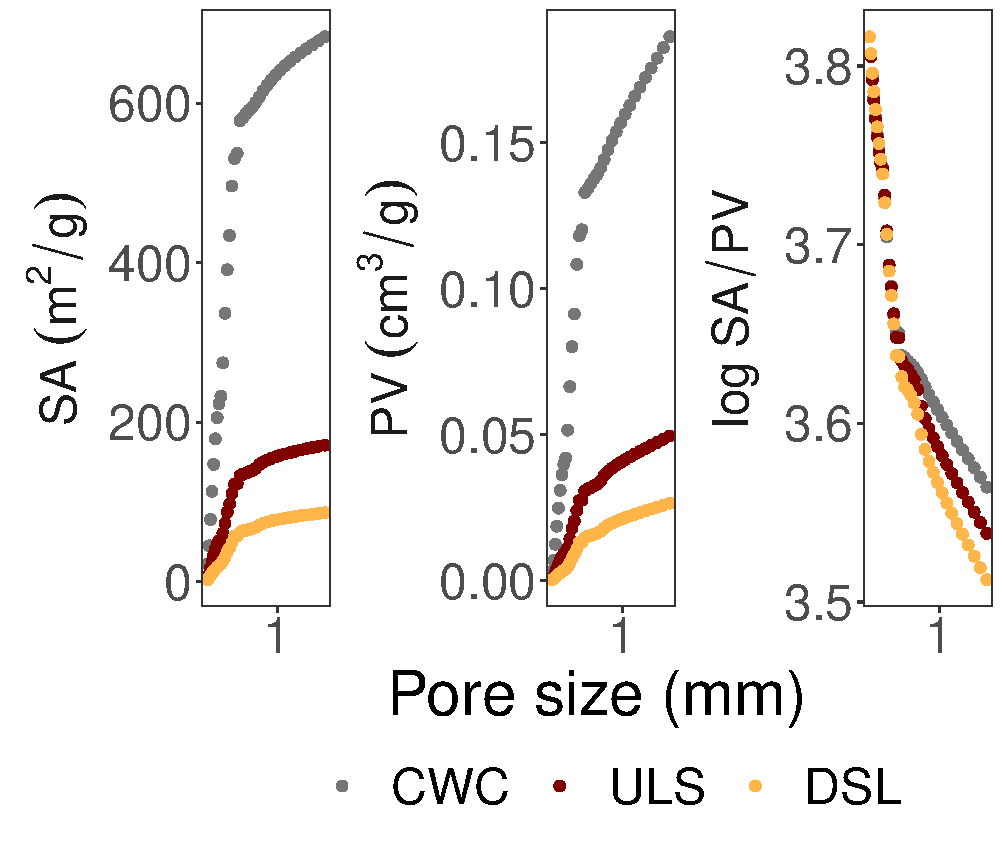
\includegraphics[width=0.8\textwidth]{R/figs/PZD_SAPV_C_small_plot.pdf}
    \caption{Cumulative pore size distribution for pores 0.4-1.5 nm using DFT.}
    \label{fig:PZD_small}
\end{figure}

\begin{table}
\caption{Effective cross-sectional diameter ($D_{eff}$) and maximum diameter ($D_{max}$) of TCs interpolated and extrapolated by linear regression from calculations performed by \cite{inoue2012size} on PFOA and other PFCAs with chain lengths 11-18.}
\centering
\begin{threeparttable}
\label{tab:molecsize}
\begin{tabular}{llll}
\toprule
Compound & Chain & $D_{eff}$ & $D_{max}$ \\ 
& length & (nm) & (nm) \\ \midrule
PFPeA & 5  & 0.45  & 0.96  \\
PFHxA & 6  & 0.50  & 1.08  \\
PFHpA & 7  & 0.56  & 1.19  \\
PFOA\textsuperscript{*} & 8 & 0.61 & 1.36 \\
PFNA & 9 & 0.67 & 1.42  \\
PFDA & 10 & 0.72 & 1.54  \\ \bottomrule                                    
\end{tabular}
\begin{tablenotes}
\item \textsuperscript{*} Value from \cite{inoue2012size}
\end{tablenotes}
\end{threeparttable}
\end{table}

\begin{figure}
    \centering
    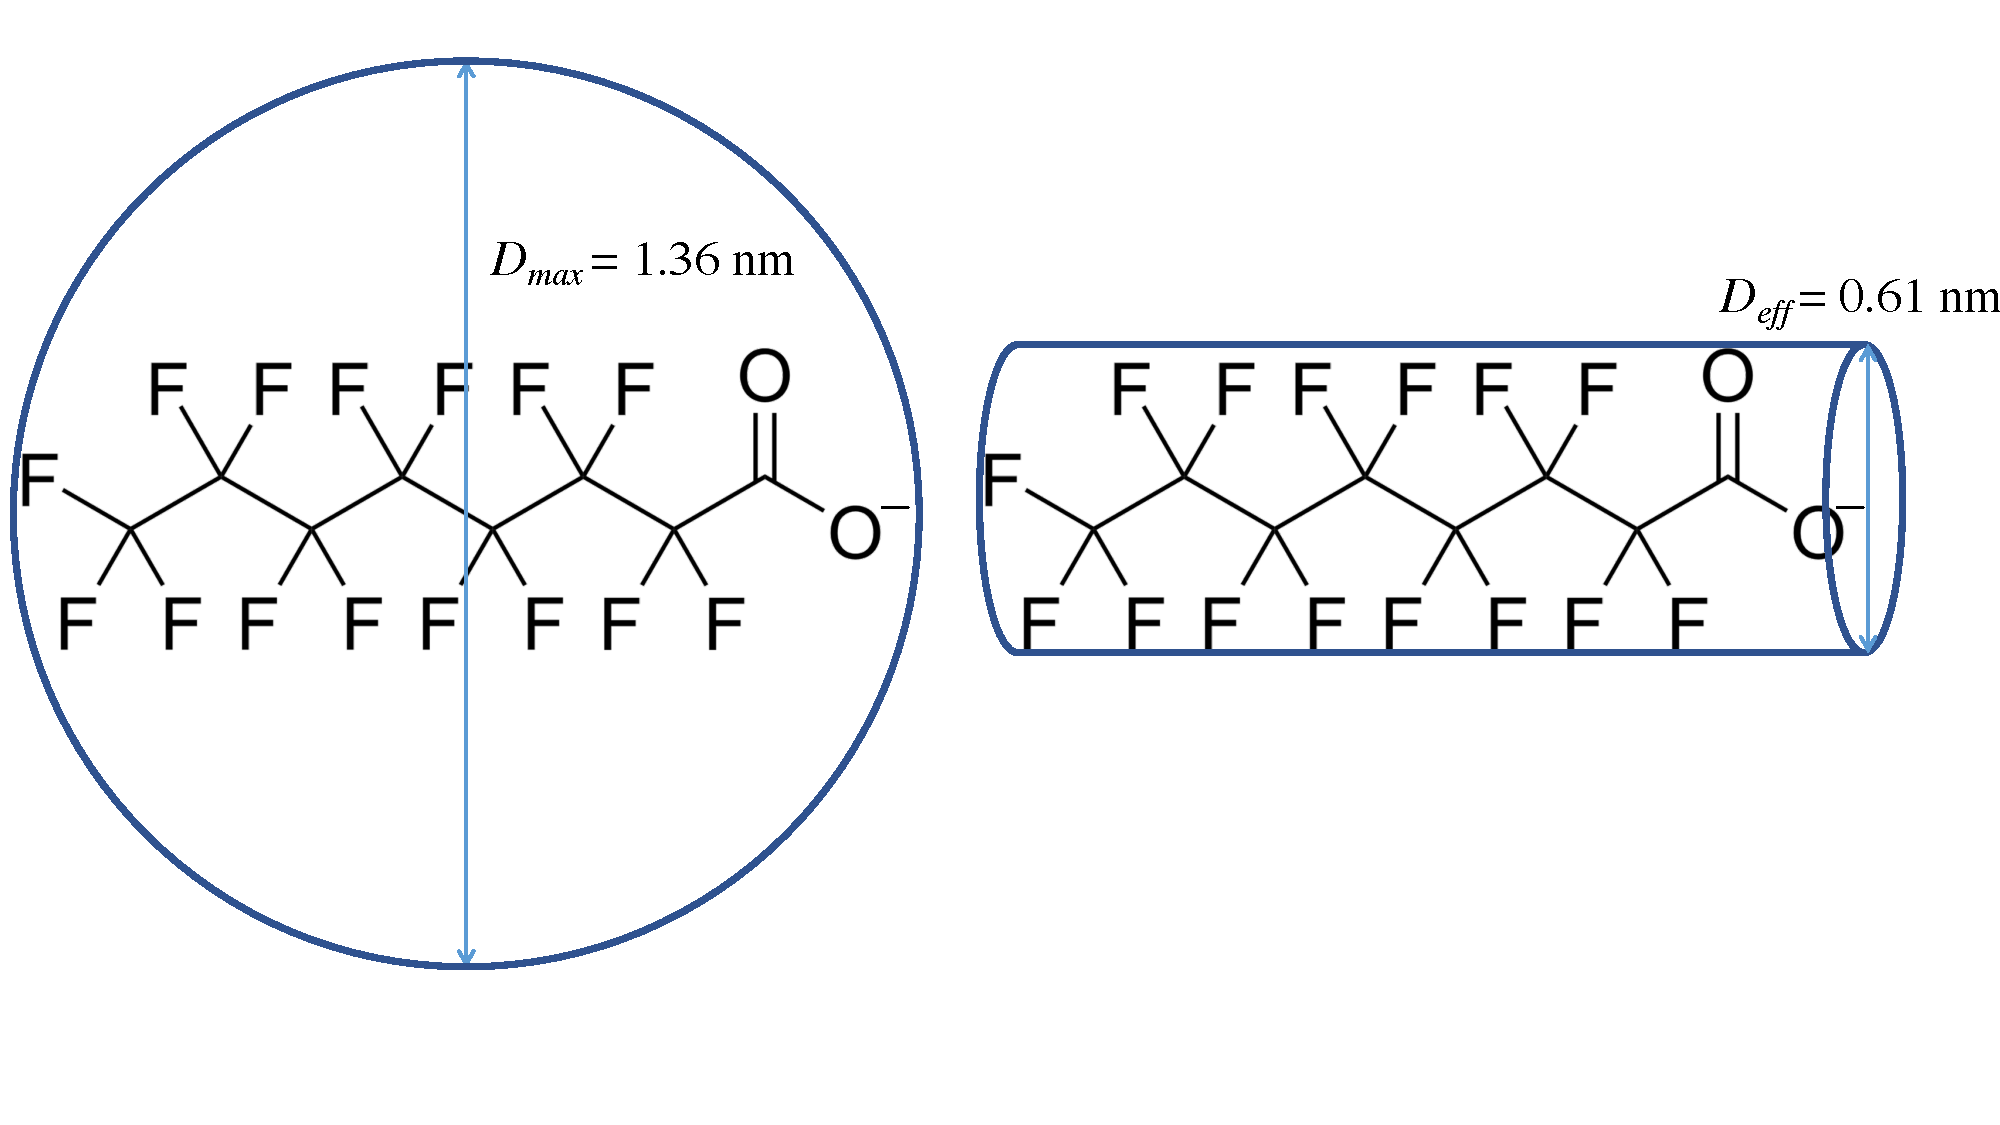
\includegraphics[width=0.8\textwidth, trim={0 2cm 0 0},clip]{Diagrams/Molecular_size.pdf}
    \caption{Definition of effective cross-sectional diameter ($D_{eff}$) and maximum diameter ($D_{max}$) shown for PFOA.}
    \label{fig:molecularSize}
\end{figure}

\subsubsection{Pore size distribution for pores $>$1.5 nm}
Similar to the trend for small pores, CWC also had the largest cumulative SA for pores $>$1.5 nm (323 m\textsuperscript{2} g\textsuperscript{-1}) versus 110 and 128 m\textsuperscript{2} g\textsuperscript{-1} for DSL and ULS, respectively. \cref{fig:PZD_large}a shows that the highest proportion of SA is allocated to pores between 1.5-5 nm for all three biochar samples. ULS had the highest cumulative PV (0.126 cm\textsuperscript{3} g\textsuperscript{-1}), whereas PV for CWC was one order of magnitude lower (0.017 cm\textsuperscript{3} g\textsuperscript{-1}). Further, the development of PV with pore size in \cref{fig:PZD_large}b shows a clear distinction between CWC and the two sewage sludge biochars. CWC has most of its PV in pores $<$3 nm, whereas ULS and DSL have volumes that increase steadily up to the maximum pore size of 35 nm. This difference becomes important when interpreting a new parameter, the SA/PV ratio, which is graphed in \cref{fig:PZD_large}c. The SA/PV better indicates the spatial arrangement of pores, where a low ratio reflects pores of maximum sorption volume. Here, ULS and DSL have low and equivalent log SA/PV ratios of 2.8 compared to CWC, which has a higher ratio of 3.21 (\cref{tab:SAPV}). Previous studies are consistent in concluding that a large internal surface area and pore volume of adsorbents is one of the most important parameters achieving high sorption capacity of PFAS \citep{du2014adsorption,Sormo2021,Hale2016,ahmed2020per}. Likewise, the results from this study provides clear indications that a low SA/PV ratio can be used to explain higher sorption capacity of ULS and DSL. Since the pores of CWC consists almost exclusively of pores $<$3 nm, whereas ULS and DSL have pores of larger size, this is the most plausible explanation for why CWC is the weakest sorbent among the three samples in this study. The shift observed by comparing SA and PV together demonstrates the importance of considering both pore size \textit{and} surface area when evaluating available sorption sites on biochar.

Since ULS and DSL have nearly equivalent SA/PV ratios, another parameter is needed to explain why ULS is a better sorbent than DSL in this study (\cref{fig:PZD_large}c). Apart from SA and PV, carbon content has shown to be a good predictor of sorption affinity to PFAS from previous literature \citep{Hale2016}. A clear distinction in pore structure emerges by by normalizing the SA/PV ratio for C-content, whereby ULS consists of 29.6 \% C versus 13.5 \% for DSL (\cref{fig:PZD_large}d). ULS has a lower (SA/PV)/C ratio, which means that the pore walls of ULS consists of a higher percentage C making the pore walls more hydrophobic and enhances sorption affinity of PFAS. 

\cref{fig:Kd_SAPV_C} also shows that individually, C and SA/PV does not explain sorption, but together they do.  

In summary, difference in sorption between CWC, DSL, and ULS can be explained by 1) difference in nanopore and micropore structure, where a higher number of large micropores signified by low SA/PV ratio is more ideal for sorption of long-chain PFASs such as PFOA, PFNA, and PFDA, and 2) a higher proportion of carbon in the pore wall matrix further enhances sorption by creating more hydrophobic sorption surfaces. Since the conclusions drawn for the sorption mechanisms contributing to PFCA sorption is based on only three biochar samples, further research within this area should test if a higher sample size comply with the suggestion that pore size size and structure is the most important determinant for sorption of organic contaminants. 

\citep{Ahmad2014}: table 3 lists sorption mechanisms found from other sorption studies, find if contaminants studied have similar size to PFAS, because properties will be very different. Many studies conclude with porosity (either nano, micro porosity and high surface area being the dominant sorption mechanisms. Adsorption due to... micro- or meso-pores Samples with large total surface area exhibit high micropore volumes, whereas samples with low total SA, generally has larger fractions of open SA (macropores) \citep{Hale2011}. 

\begin{figure}[htb]
    \centering
    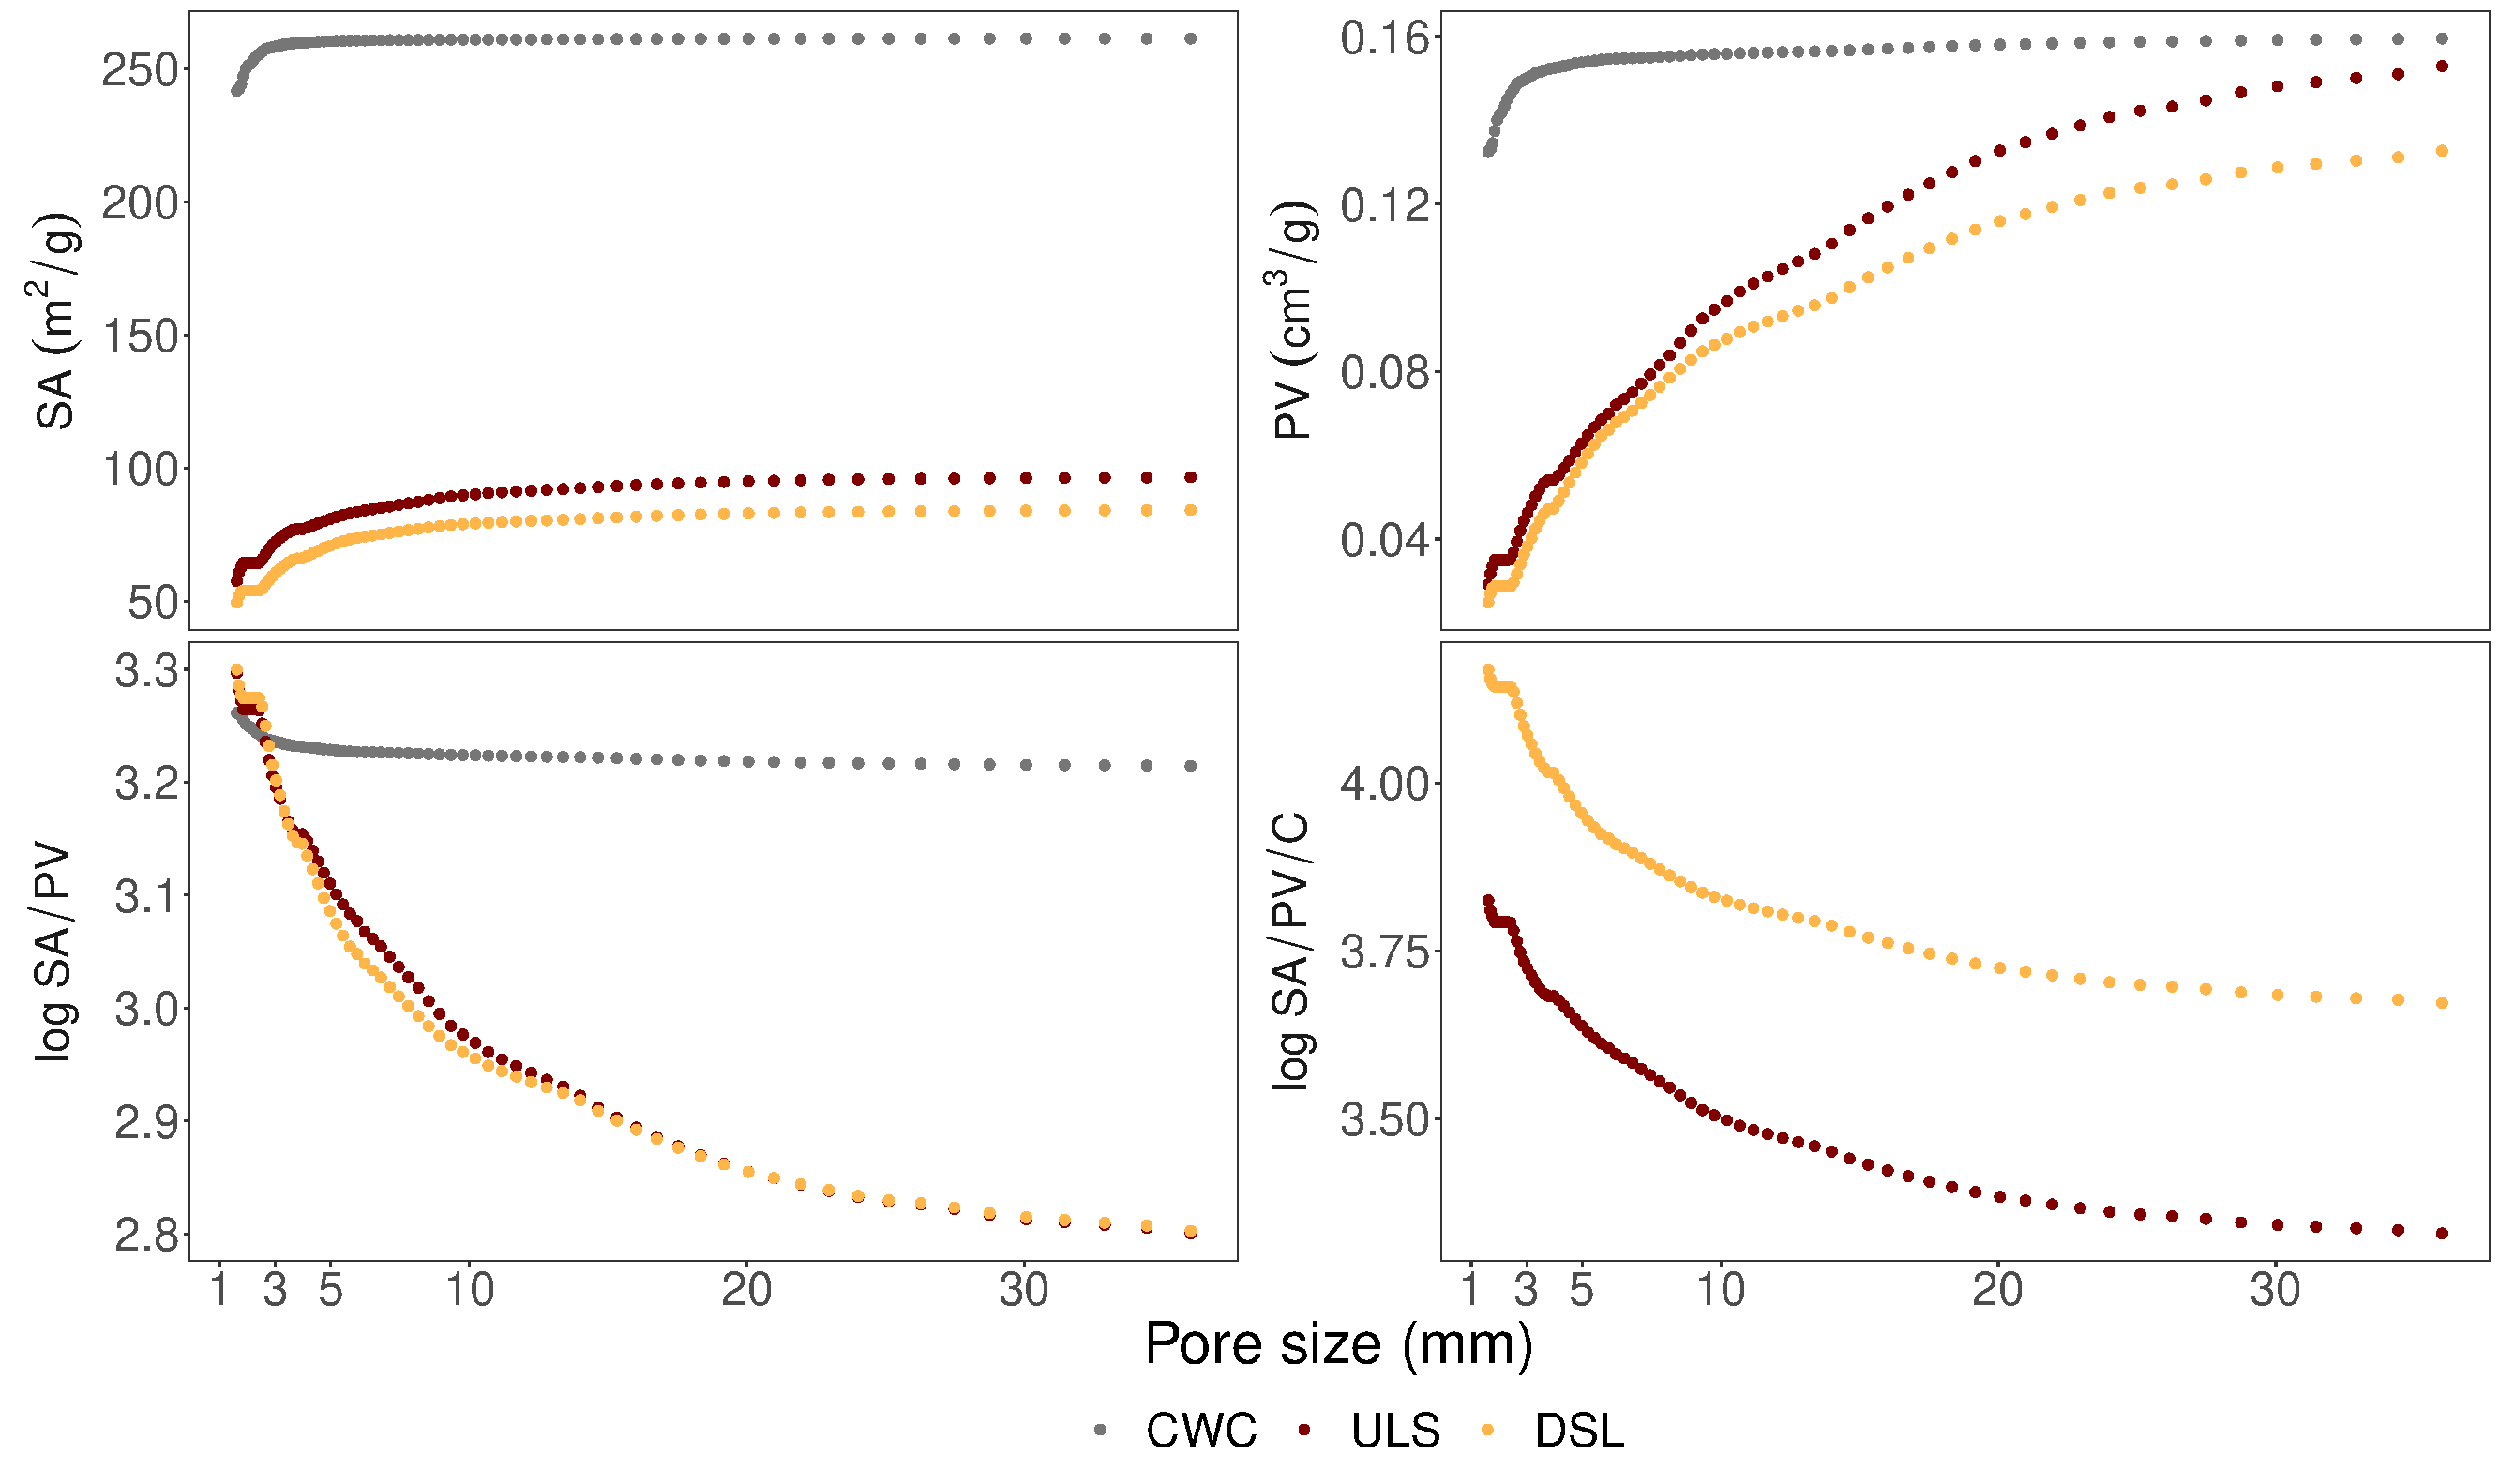
\includegraphics[width=\textwidth]{R/figs/PZD_SAPV_C_large.pdf}
    \caption{Cumulative pore size distribution for pores $>$ 1.5 nm using DFT theory. (a) Surface area, (b) pore volume, (c) SA/PV ratio for pores $>$1.5 nm normalized to carbon content (g C/g BC). (d) A lower SA/PV/C ratio indicates a higher degree of C in the pore wall matrix.}
    \label{fig:PZD_large}
\end{figure}

\subsection{Surface chemistry}
Based on feedstock type for the three biochars studied in this thesis, carbon content of the biochars follows the expected trend, CWC \textless ULS \textless DSL with 91.4\%, 29.6\% and 13.5\%, respectively (\cref{tab:SAPV}). Oxygen content was highest for DSL and ULS (61.4 and 57.1 \% respectively) compared to 5.5 \% for CWC. CWC has a low O/C and H/C ratio (\textless 1) whereas ULS and DSL have ratios \textgreater 1. A low H/C and O/C ratio is associated with high degree of aromaticity and few functional groups. This shows that the CWC matrix is dominated by aromatic carbon whereas ULS and DSL are dominated by oxidized carbon resulting in a more hydrophobic surface of the high-C biochar. A high degree of aromaticity have been reported in previous literature to be important for sorption of hydrophobic organic contaminants such as PAH's \citep{Cornelissen2005}. However, \cite{du2014adsorption} report that a higher O/C ratio with a biochar matrix consisting of more surface functional groups that are Lewis acids (hydroxyl, carbonyl, and metal-containing groups) have been found to be beneficial for sorption because they aid in the diffusion of PFAS into deeper pores that increases sorption capacity. The reason for this is that the CF chain is net negative and ion bridging is important because biochar is accompanied with high ash contents containing divalent cations. This interaction is stronger than hydrophobic interaction, which is only a compromise for PFAS which is more hydrophobic than oleophobic. It can hypothesized that the higher O/C ratio of the sewage sludge biochars may then be a contribution factor for stronger sorption seen for these chars. Although sorption capacity has not been measured directly, this might indicate that sorption at more inaccessible sites occur on the sludge biochars by the aid of surface functional groups. 

The proportion of elements other than C, O, H and N contained in the biochar matrices is significantly lower for the clean wood biochar (1.4 \%) compared to the sludge biochars (10.9 and 23.2 \%), containing a greater mixture of other elements. Total elemental composition of the biochars is given in \cref{appSec:elements}. The results from this study is in contrast to literature \citep{Hale2016,Sormo2021,zhang2021sorption} that report that the sorption strength of organic compounds to biochar increases with decreasing biochar O/C and biochar H/C ratios. Thus, the higher sorption onto ULS and DSL cannot be explained by the sorbent composition of main elements alone.

\cite{du2014adsorption} summarizes that the more basic groups the adsorbents have, the more PFAS they can adsorb, which is somewhat counter intuitive when considering potential repulsion by the anionic PFCA functional group. The reason for this is that these groups are typically weak acids that are prone to be protonated at environmentally relevant pH's. A high pH-point of zero charge (PZC) therefore increases the adsorption capacity because the surface functional groups are more likely to be protonated. A high nitrogen/carbon (N/C) ratio is a predictor of amine groups, which is positively charged, where the N/C ratios for the biochars are listed in \cref{tab:SAPV}. Both ULS and DSL have higher ratios than CWC by one order of magnitude, so this could be a contributing factor to why the sewage sludge biochars are better sorbents for PFCAs. Even though total N does not indicate amine groups, this is an indication. Not much is known about what happens to proteins etc. during pyrolysis and how this affects speciation. But common is that this char type is more nutrient rich, which proves to be beneficial for sorption of PFAS in this study. Biochar consists of poly-condensed aromatic rings which make the surface \textpi-electron dense, called graphitized surface. Has the ability to bind electron-withdrawing molecules by being \textpi-electron donor. (ring condensation increases with pyrolysis temperature of biochar) PFAS cannot undergo pi interactions because surface also is net negative \citep{Li2019} Literature says that pi pi EDA is an important sorption mechanism between aromatic rings (pi electron donor) and amides (pi electron acceptor). It can be hypothesized that the electron donor/acceptor role can be switched by sorption or PFAS to sludge char which has a high N/C ratio, that could be attributed to amide groups situated in the benzene rings \citep{Li2019}

Adsorption capacity has shown to also be related to solution pH, which is expected to increase with decreasing pH \citep{du2014adsorption}. However, in Ca and Mg-rich basic solutions, sorption can be enhanced through divalent cation bridging effect. pH varied little between all biochar-soil-water systems with an average pH of 7.18 \textpm 0.02. Conductivity was 39 \textpm 0.9 \textmu S cm\textsuperscript{-1}. Since the variance is low, pH and conductivity was not considered as factors that influence sorption of PFCAs. The conductivity of soil-water samples differed the most from the rest of the samples with a mean conductivity of 23 \textpm 0.05 \textmu S cm\textsuperscript{-1} versus a mean of 41 \textpm 0.9 \textmu S cm\textsuperscript{-1} for the biochar-water and biochar-soil-water samples. Complete pH and conductivity data is in \cref{appSec:misclab}.

\citep{zhang2013sorption}: sorption of PFAS increases with decreasing pH
Biochar charge morphology of functional groups are influenced by solution pH, deprotonation and protonation of functional groups, depends on environmental conditions \citep{Li2019}. Influences adsorption ability of environmental contaminants depending on surface morphology, especially hydrophobicity. In terms of PFCAs, biochar is expected to be a better sorbent at low pH due to limitation of electrostatic repulsion of biochar functional groups and the polar head of the perfluoroalkyl carboxylate. 

\begin{table}
\centering
\caption{Mean pH and conductivity (\textmu S cm\textsuperscript{-1}) measurements for the different batch test systems (n=3). The error bars represent the standard error. BC/S/L is the biochar:soil:liquid ratio.}
\label{tab:pHcond}
\begin{tabular}{lccccc}
\toprule
 & \multicolumn{2}{c}{pH} & \multicolumn{2}{c}{Conductivity} & \\ \cline{2-5}
 & mean & std. dev & mean & std. dev & BC/S/L\\ 
\midrule
ULS & 7.10 & 0.04 & 45.70 & 3.03 & 1/0/500\\
DSL & 7.31 & 0.02 & 40.93 & 1.07 & 1/0/500\\
CWC & 7.36 & 0.07 & 46.47 & 0.70 & 1/0/500\\
ULS+S & 7.18 & 0.02 & 34.93 & 0.40 & 1/50/500\\
DSL+S & 7.14 & 0.00 & 35.73 & 1.50 & 1/50/500\\
CWC+S & 7.09 & 0.05 & 44.90 & 1.54 & 1/50/500\\
S & 7.08 & 0.05 & 23.33 & 0.87 & 0/1/10\\
\bottomrule
\end{tabular}
\end{table}

\begin{figure}[htb]
    \centering
    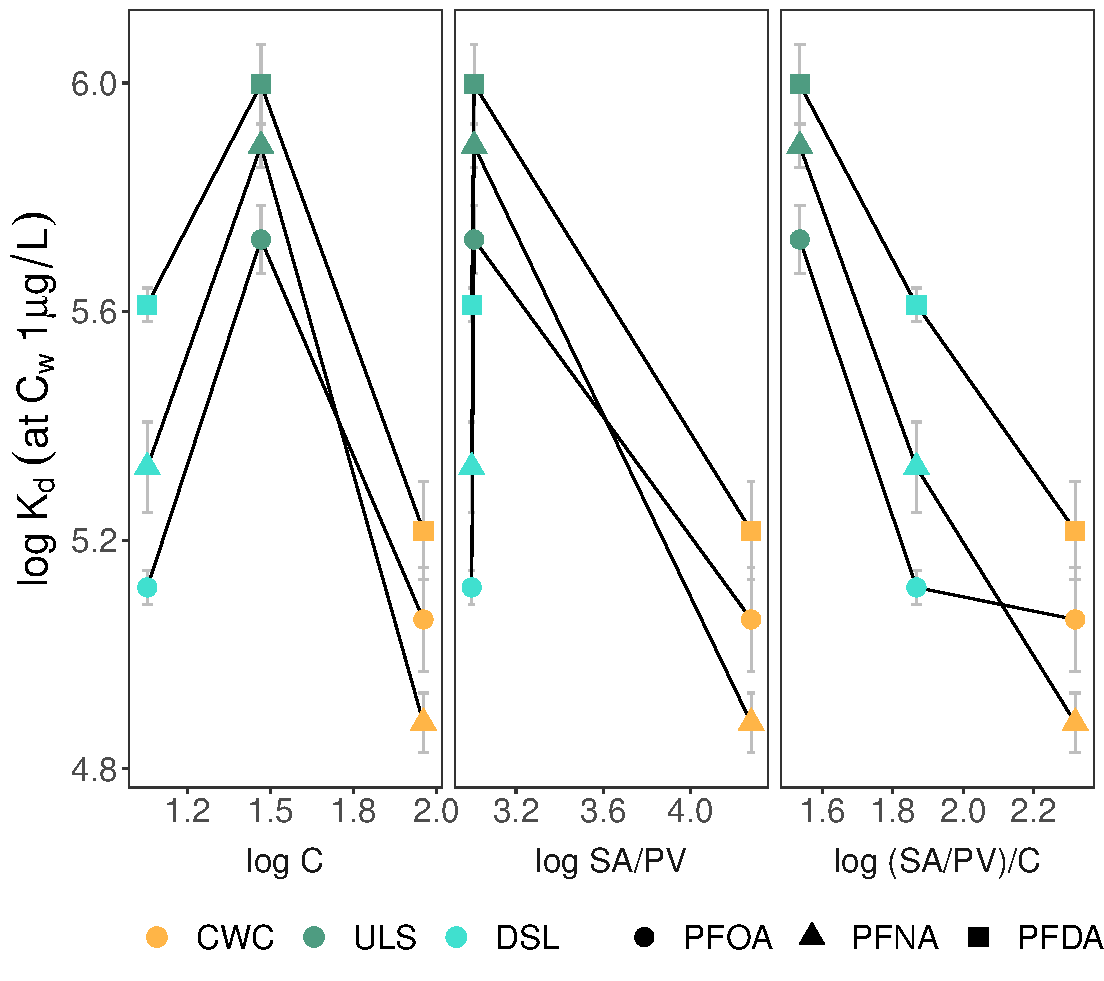
\includegraphics[width=0.8\textwidth]{R/figs/SAPV_C_Kd1ugL_plot.pdf}
    \caption{The correlation of $log~K_d$ vs. (a) log C (b) log SA/PV (c) log (SA/PV)/C using BET for SA and BJH for PV by biomass feedstock. Error bars are the propagated standard error of $log~K_F$ and $n$.}
    \label{fig:Kd_SAPV_C}
\end{figure}


\subsection{Effect of solution chemistry}

\begin{table}
\centering
\caption{Composition of a selection of elements in the biochar samples in mg/kg.}
\label{tab:BC_mainElements}
\begin{tabular}{lllllllll} \toprule
 & Ca & Fe & K & Mg & Na & P & S & Si \\ \midrule
CWC & 8.03 & 0.13 & 4.0 & 0.91 & 0.052 & 0.41 & 0.089 & 0.17 \\
DSL & 26 & 180 & 3.7 & 4.7 & 1.8 & 8.0 & 7.2 & 0.62 \\
ULS & 21 & 23 & 6.8 & 5.3 & 2.4 & 45 & 2.9 & 1.7 \\ \bottomrule
\end{tabular}
\end{table}

\subsection{Effect of inorganic ions}
Elements that may affect sorption properties of the biochars are provided in \cref{tab:BC_mainElements}. Since ionic forms have not been analyzed, an assumption based on the total element composition must be made during the discussion of potential roles of inorganic ions for PFAS sorption. The sludge chars have expectantly the highest mineral content overall due to the heterogeneous composition of sewage sludge. 
Coexisting inorganic cations and anions complicates sorption behavior of PFCAs, where several mechanisms are involved in changing both solution and biochar surface chemistry \citep{du2014adsorption}. The presence of ions can both enhance or suppress sorption through mechanisms such as electrical double-layer compression, surface-charge neutralization, divalent cation bridging, competitive adsorption, and salting-out. The latter mechanism occurs only at high enough salt concentration and is not applicable for the present study. 

ULS and DSL are similar in earth alkali composition that gives rise to divalent ions  and CWC is one and two orders of magnitude lower in Ca and Mg, respectively. The presence of electrolytes creates an electrical double layer (EDL) that changes the adsorption surface. Divalent ions such as Ca\textsuperscript{2+} and Mg\textsuperscript{2+} in the EDL can function as bridges between the negatively charged functional groups of PFAS and surface negative charges. This divalent cation bridging effect has shown to be an important sorption mechanism in sediments, mineral materials, and black carbon, among others \citep{higgins2006sorption}. Apart from playing a bridging role between the BC surface and PFAS functional groups, divalent ions can function as intermolecular PFAS bridges which further enhances PFAS hydrophobicity by this complexation into larger molecules. Both Ca\textsuperscript{2+} and Mg\textsuperscript{2+} have been reported to play a role for chaining of perfluorinated carboxylic acids \citep{wang2011}. The role of divalent cations  

Increase in zeta potential 

Previous research suggests that calcium content is an important parameter contributing to stronger sorption of anionic organic molecules \citep{higgins2006sorption,sigmund2022sorption}. In this study, PFAS sorption to sludge enhanced with increasing calcium concentration in solution, divalent ions contribute to stronger sorption compared to monovalent ions due to ion bridging between negatively charged PFAS and biochar at low pH \citep{zhang2013sorption,arvaniti2014sorption,arvaniti2015review}. 

\begin{figure}[htb]
    \centering
    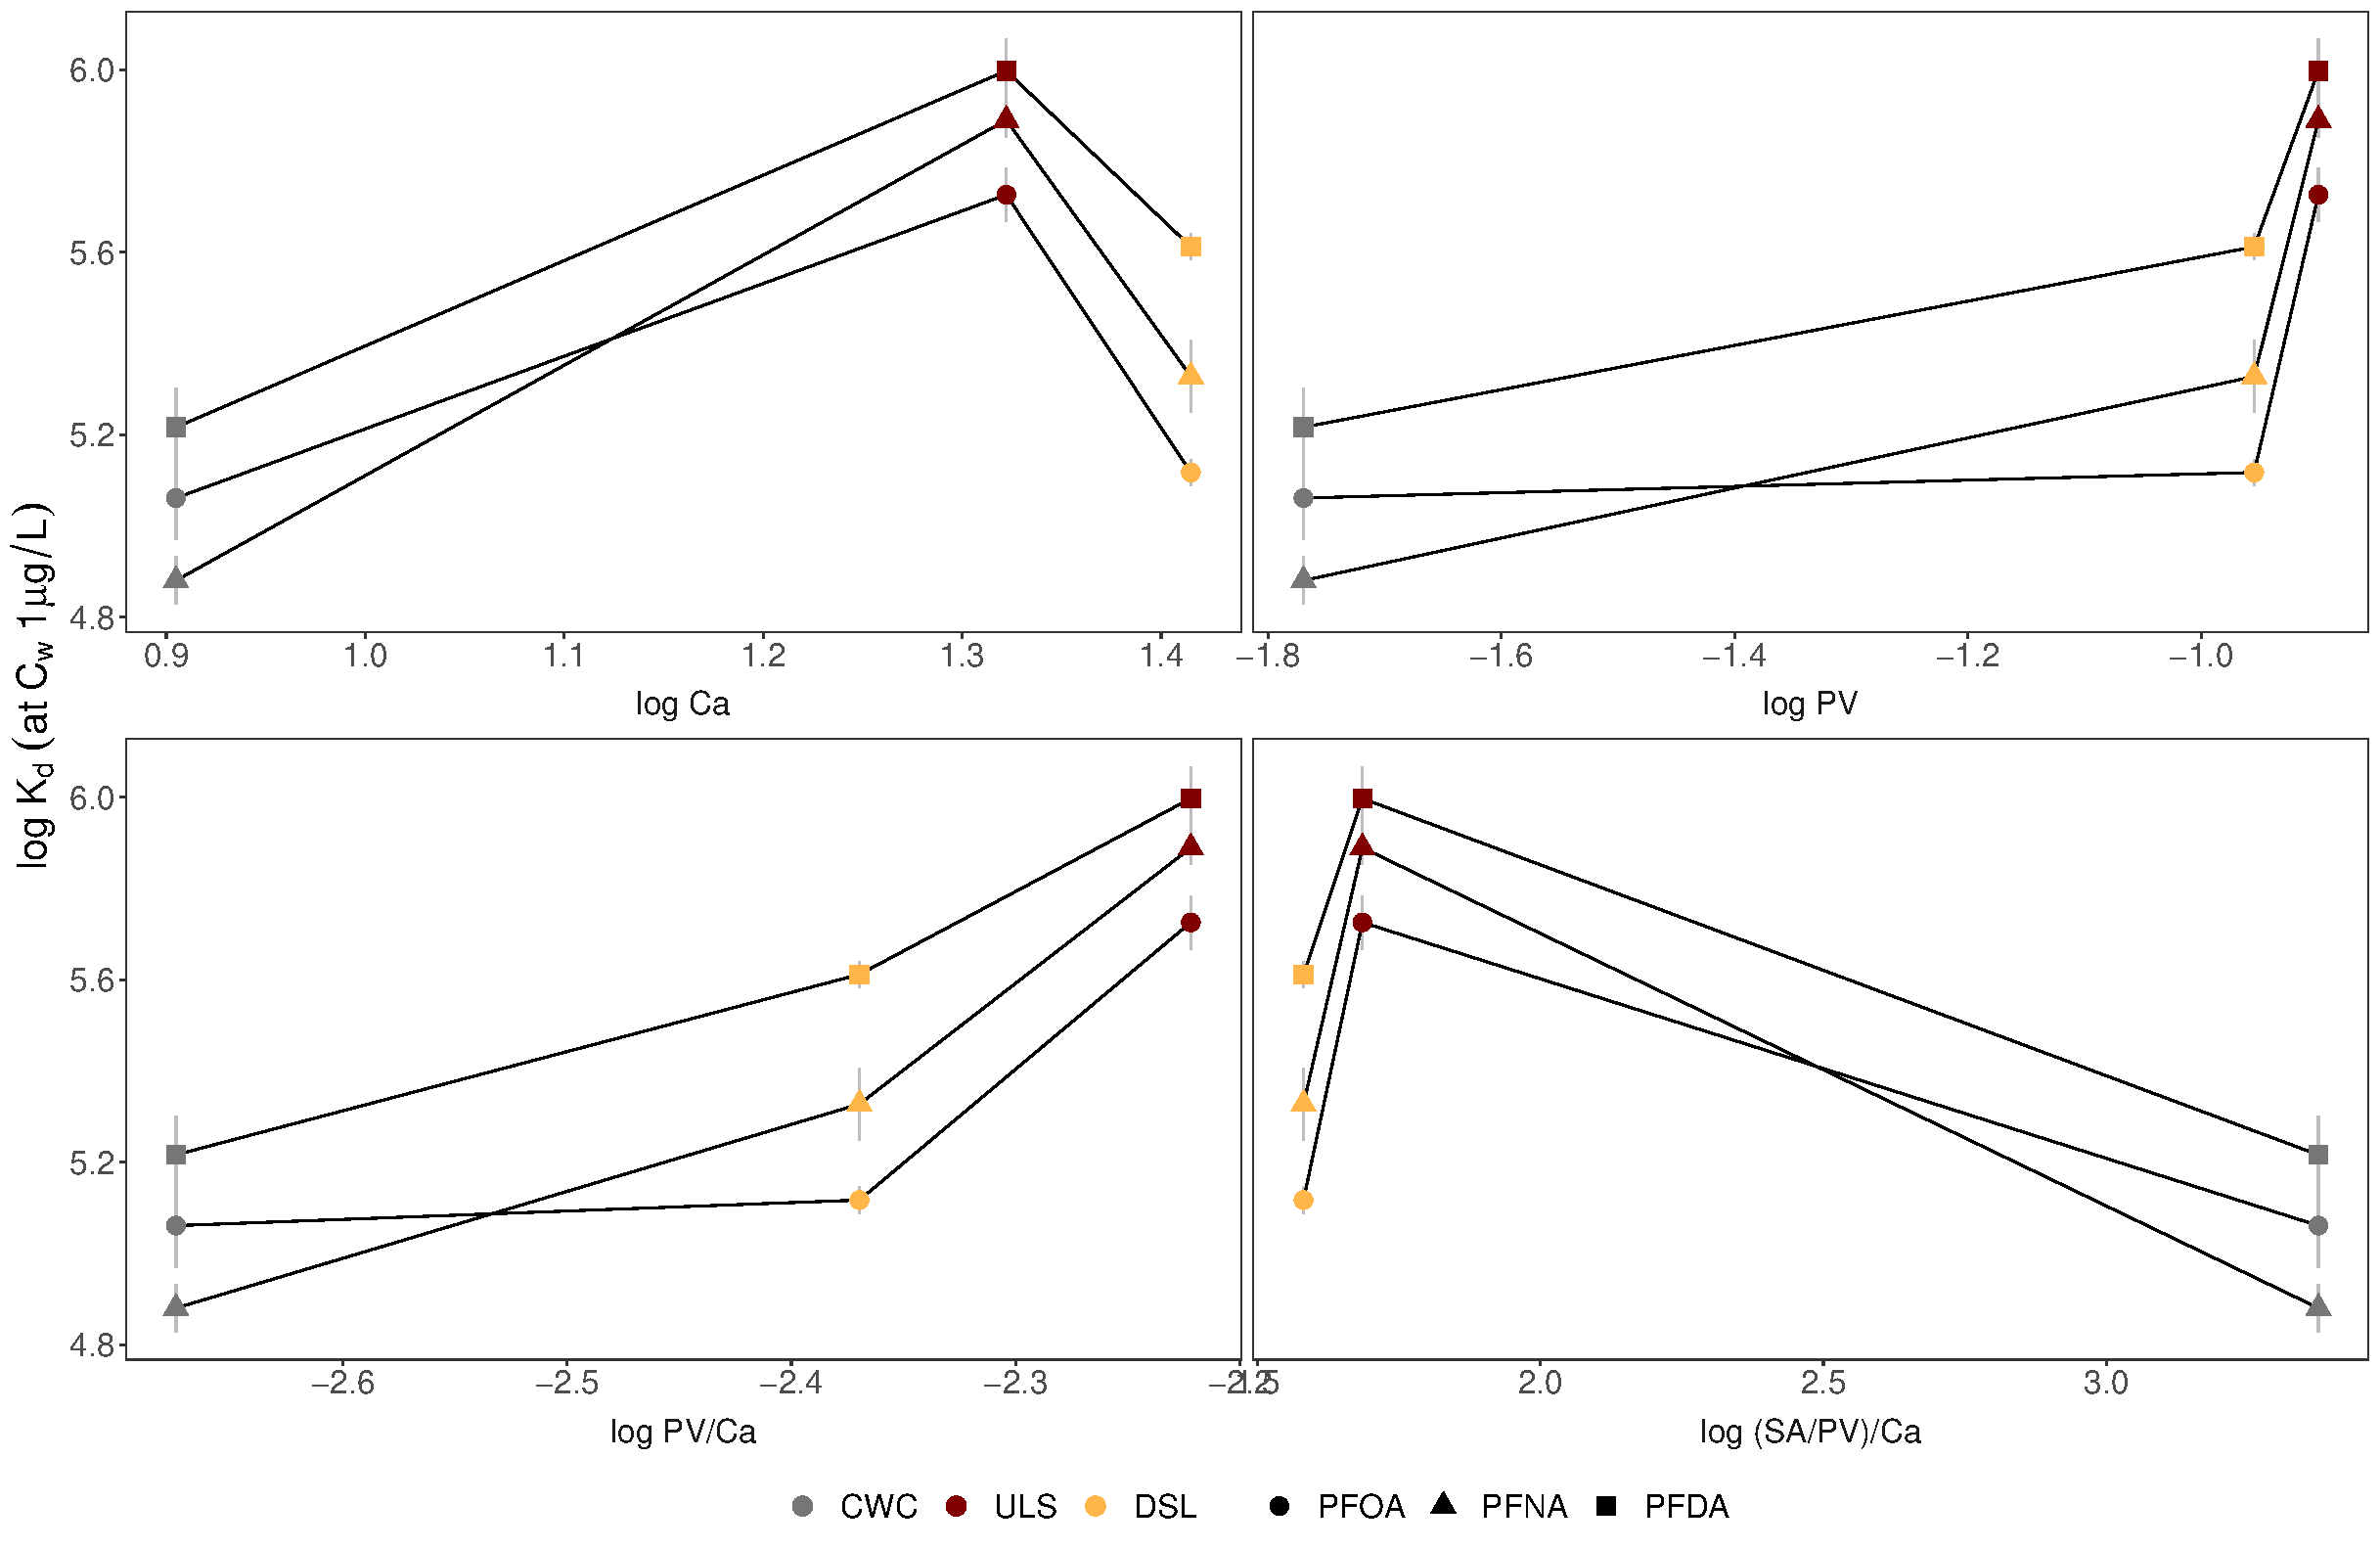
\includegraphics[width=0.8\textwidth]{R/figs/Correlation_SAPV_Ca_plot.pdf}
    \caption{The correlation of $log~K_d$ vs. (a) log Ca (b) log PV (c) log PV/Ca (d) log (SA/PV)/Ca using BET for SA and BJH for PV by biomass feedstock. Error bars are the propagated standard error.}
    \label{fig:Kd_SAPV_Ca}
\end{figure}

\subsubsection{Iron speciation}
Iron in the biochar matrix is not only present as iron oxides, but unknown species. Due to the lack of corresponding reference compounds for these species, no satisfying fit was obtained for the iron species present in the sewage sludge biochar samples. 
Iron speciation, Synchrotron results, Inner-sphere complexes (covalent metal-ligand bonds) with Fe-carboxylate by ligand exchange \citep{gao2012adsorption}(NEED TO GET ACCESS TO ARTICLE, BUT CITED IN \citep{du2014adsorption}):

\begin{equation}
    \mathrm{\equiv Fe-OH_2^+~ + ~ CF_3(CF_2)_nCOO^- \rightarrow   ~ \equiv Fe-OOC(CF_2)_nCF_3 ~+~ H_2O}
\end{equation}

Gabrielle: point of zero charge (pzc) for Fe(oxyhydr)oxides such as ferrihydrite and goethite are around 7. which is the same solution pH measured for the biochar solutions so iron species are expected to be neutral for the systems analyzed (\cref{tab:pHcond}). However, this is not certain because other iron species present could not be identified. 

Fe valence: results from XANES show that DSL and ULS are similar in valence and speciation and consist of mostly reduced forms of Fe (Fe(II)), where DLS is slightly more reduced than ULS, but how much is not quantified. 

%%%%%%%%%%%%%%%%%%%%%%%%%%%%%%%%%%%%%%%%%%%%%%%%%%%%%%%%%%%%%%%%%%%%%%%%%%%%%%%%%%%%%%%%%%%%%%%%%%%%%%%%%%%%%%%%%%%%%
%%%%%%%%%%%%%%%%%%%%%%%%%%%%%%%%%%%%%%%%%%%%%%%%%%%%%%%%%%%%%%%%%%%%%%%%%%%%%%%%%%%%%%%%%%%%%%%%%%%%%%%%%%%%%%%%%%%%%
%%%%%%%%%%%%%%%%%%%%%%%%%%%%%%%%%%%%%%%%%%%%%%%%%%%%%%%%%%%%%%%%%%%%%%%%%%%%%%%%%%%%%%%%%%%%%%%%%%%%%%%%%%%%%%%%%%%%%

\section{Sorption attenuation PFCA cocktail and soil}
\cref{subfig:C10} shows the $K_d$-values for the different batch test categories (BC single, BC soil single, BC soil mixed, BC mixed, soil single, and soil mixed) spiked with the same concentration of each compound at the highest spike point, SC10 (\cref{tab:spikeConcentrations}). $K_d$ for the biochar-soil batch tests have not been corrected for the amount sorbed by soil itself due to inconsistent results for the $K_d$ in soil (see \cref{appSec:Sorption}, \cref{apptab:attenuation} for soil $K_d$'s). Therefore, $K_d$ for BC soil single, BC soil mixed and BC mixed represent the partitioning coefficients for biochar and soil altogether. The sandy soil used has poor sorption affinity with a mean $log~K_d$ value of 2.47 versus $log~K_d$ of, for example, 6.06 for singly-spiked PFDA to ULS-water. The total concentration of C5-C10 spiked at SC10 was 7.8 mg/L for the BC cocktail and 10.8 mg/L for the BC soil cocktail. The 3 mg/L difference between the two is because the cocktail batch tests were spiked in two different ways (described in \cref{sec:S-BC}. The cocktail consisted of 2.5\% PFPeA, 7.7\% PFHxA, 1.4\% PFHpA, 18.2\% PFOA, 21.3\% PFNA, and 48.8\% PFDA. Since different concentrations of each compound were used to make the cocktail solution, a trend for attenuation with chain length cannot be derived. However, the relative $K_d$-values of each batch test category as well as comparisons between biochar samples provides for an interesting discussion. This way of comparing $K_d$-values was decided to be the most straight forward way of comparing partitioning of the same compound across biochar samples because the same amount of PFCAs have been added to the system.

In \cref{subfig:C10}, the drop in $log~K_d$ from $log~K_d$ for BC single represents how much the resulting partition coefficient for each batch test category is affected by the presence of soil and a PFCA cocktail. For all compounds, the presence of a mixture contributes to the highest drop in $log~K_d$. Overall, $log~K_d$ decreases in the following order: BC single $>$ BC soil single $>$ BC soil mixed $>$ BC mixed $>$ soil single and mixed. Attenuation appears to be similar for all biochars as the points for each batch type align parallel, at least for the more consistent results for PFOA, PFNA, and PFDA. This trend shows that the mixed systems have the greatest attenuation, where sorption is up to two orders of magnitude weaker than the reference. This means that sorption is non-linear at high concentrations, which will be discussed further in \cref{sec:non-linearity}. These results are in accordance with previous literature \citep{deng2010removal,zhou2010sorption}.

\cref{subfig:AF} shows the attenuation factors (AF) for each batch test category, which is defined as: 

\begin{equation} \label{eq:AF}
    AF = \frac{K_{d,x}}{K_{d,BC single}}
\end{equation}

where the numerator $K_{d,x}$ are the mixed, soil mixed, or soil single batch test sample partition coefficients. It appears that attenuation by a cocktail in soil and biochar only is within the range  of maximum sorption capacity with little variance between the biochar samples. compared to the biochar-water single-spike batch tests. AFs for PFPeA, PFHxA and PFHpA were removed due to the lack of consistent results, and sorption was reduced with $\ge$99\% ranging from 35\% of expected sorption for CWC-soil-PFOA down to below 15\% for the mixed samples. Strongest sorption is, as expected, for the single-spiked batch tests with biochar only. BC soil cocktail has the highest sorption attenuation, which is plausible because both soil and competing PFCAs disrupt optimal sorption.  A table of attenuation factors for each batch test category is provided in \cref{apptab:attenuation}.

It appears that ULS, which has the highest sorption, also has the highest attenuation. This phenomenon has two possible explanations: 1) the most attractive sorption sites on ULS are limited and easily blocked, and 2) in addition to the strong competition for the most attractive sorption sites described in 1), the reported $K_d$-values for the batch tests with soil are average values for sorption of biochar and soil together. The closer the sorption of the char is to the soil, the less the apparent attenuation effect. Since ULS has the highest difference in $K_d$ compared to the soil, attenuation becomes 

\cref{fig:C10_AF} show that attenuation by soil is less important than the cocktail effect. However, there is no clear distinction between BC soil mixed and BC mixed. This may be attributed to that the cocktail effect overshadows attenuation by soil. Again, this would mean that soil, which has a $log~K_d$ of 2.6 $\pm$ 2.0 sorbs some of the PFCAs that have been blocked from sorption onto the biochar. 
Colored filtrate and humus aggregation seen during analysis of the soil batch tests indicate that co-sorption to organic matter (OM) in the BC-soil-water batch test (see \cref{sec:S-BC}. The soil used was a sandy soil with 1.3 \% TOC (details on soil properties is in \cref{sec:Soil}). By the co-existence of OM and dissolved organic carbon (DOC), sorption attenuation occurs by 1) competitive and weaker sorption of PFAS on OM and DOC, and 2) competitive sorption of OM to pore walls which clogs the pores by the large humic acids (300-600 nm) that prevents diffusion of PFAS into pores \citep{Cornelissen2006,kluvcakova2018size}. Rather than the soil contributing additional sorption capacity, soil attenuates the effect of the biochar sorbents by pore clogging and competitive sorption to pore walls than enhancing sorption by the presence of additional sorbent substrate because DOC keeps some PFCAs still in solution \citep{Li2019}. Further, size of the organic molecules matter as humic molecules with similar size to PFAS contribute to highest competition \citep{du2014adsorption}, however, humic acid size fractionation was not investigated in this study.

Interaction of fouling and time: given enough time, fouling is less \citep{Werner2006}. Functional groups are typically located on the external part of biochar which can hydrogen bond with surface groups on humus preventing hydrophobic contaminants from entering the pores. Coating by humic material in high TOC soil, pore blocking \citep{Hale2011}. Describe importance of soil type, i.e., organic matter content in soil for effective sorption
Sorption generally decreases with increasing pH due to electrostatic repulsion between negatively charged surfaces and negatively charged PFAS \citep{du2014adsorption}. Cation bridging effect in high pH by presence of divalent ions such as Mg2+ and Ca2+, increases sorption even at high pH \citep{du2014adsorption}. Relevant for adsorption to sediment, black carbon. "Competition: inorganic anions can compete with anionic PFCs for adsorption sites, resulting in a decrease of PFCs sorption on adsorbents" \citep{du2014adsorption}. 
\citep{Sormo2021}: OM can weaken sorption to biochar due to pore blocking. One might think that soil high in organic matter will be strengthen sorption when amending the soil with biochar, however, this turns out to be the opposite. Refer to figure from \citep{Cornelissen2005}. Organic matter competes as sorption sites for PFAS but the sorption strength is weaker so desorption will occur more easily than once sorbed to biochar. 

\begin{figure}
    \centering
        \begin{subfigure}[]{\linewidth}
            \centering
            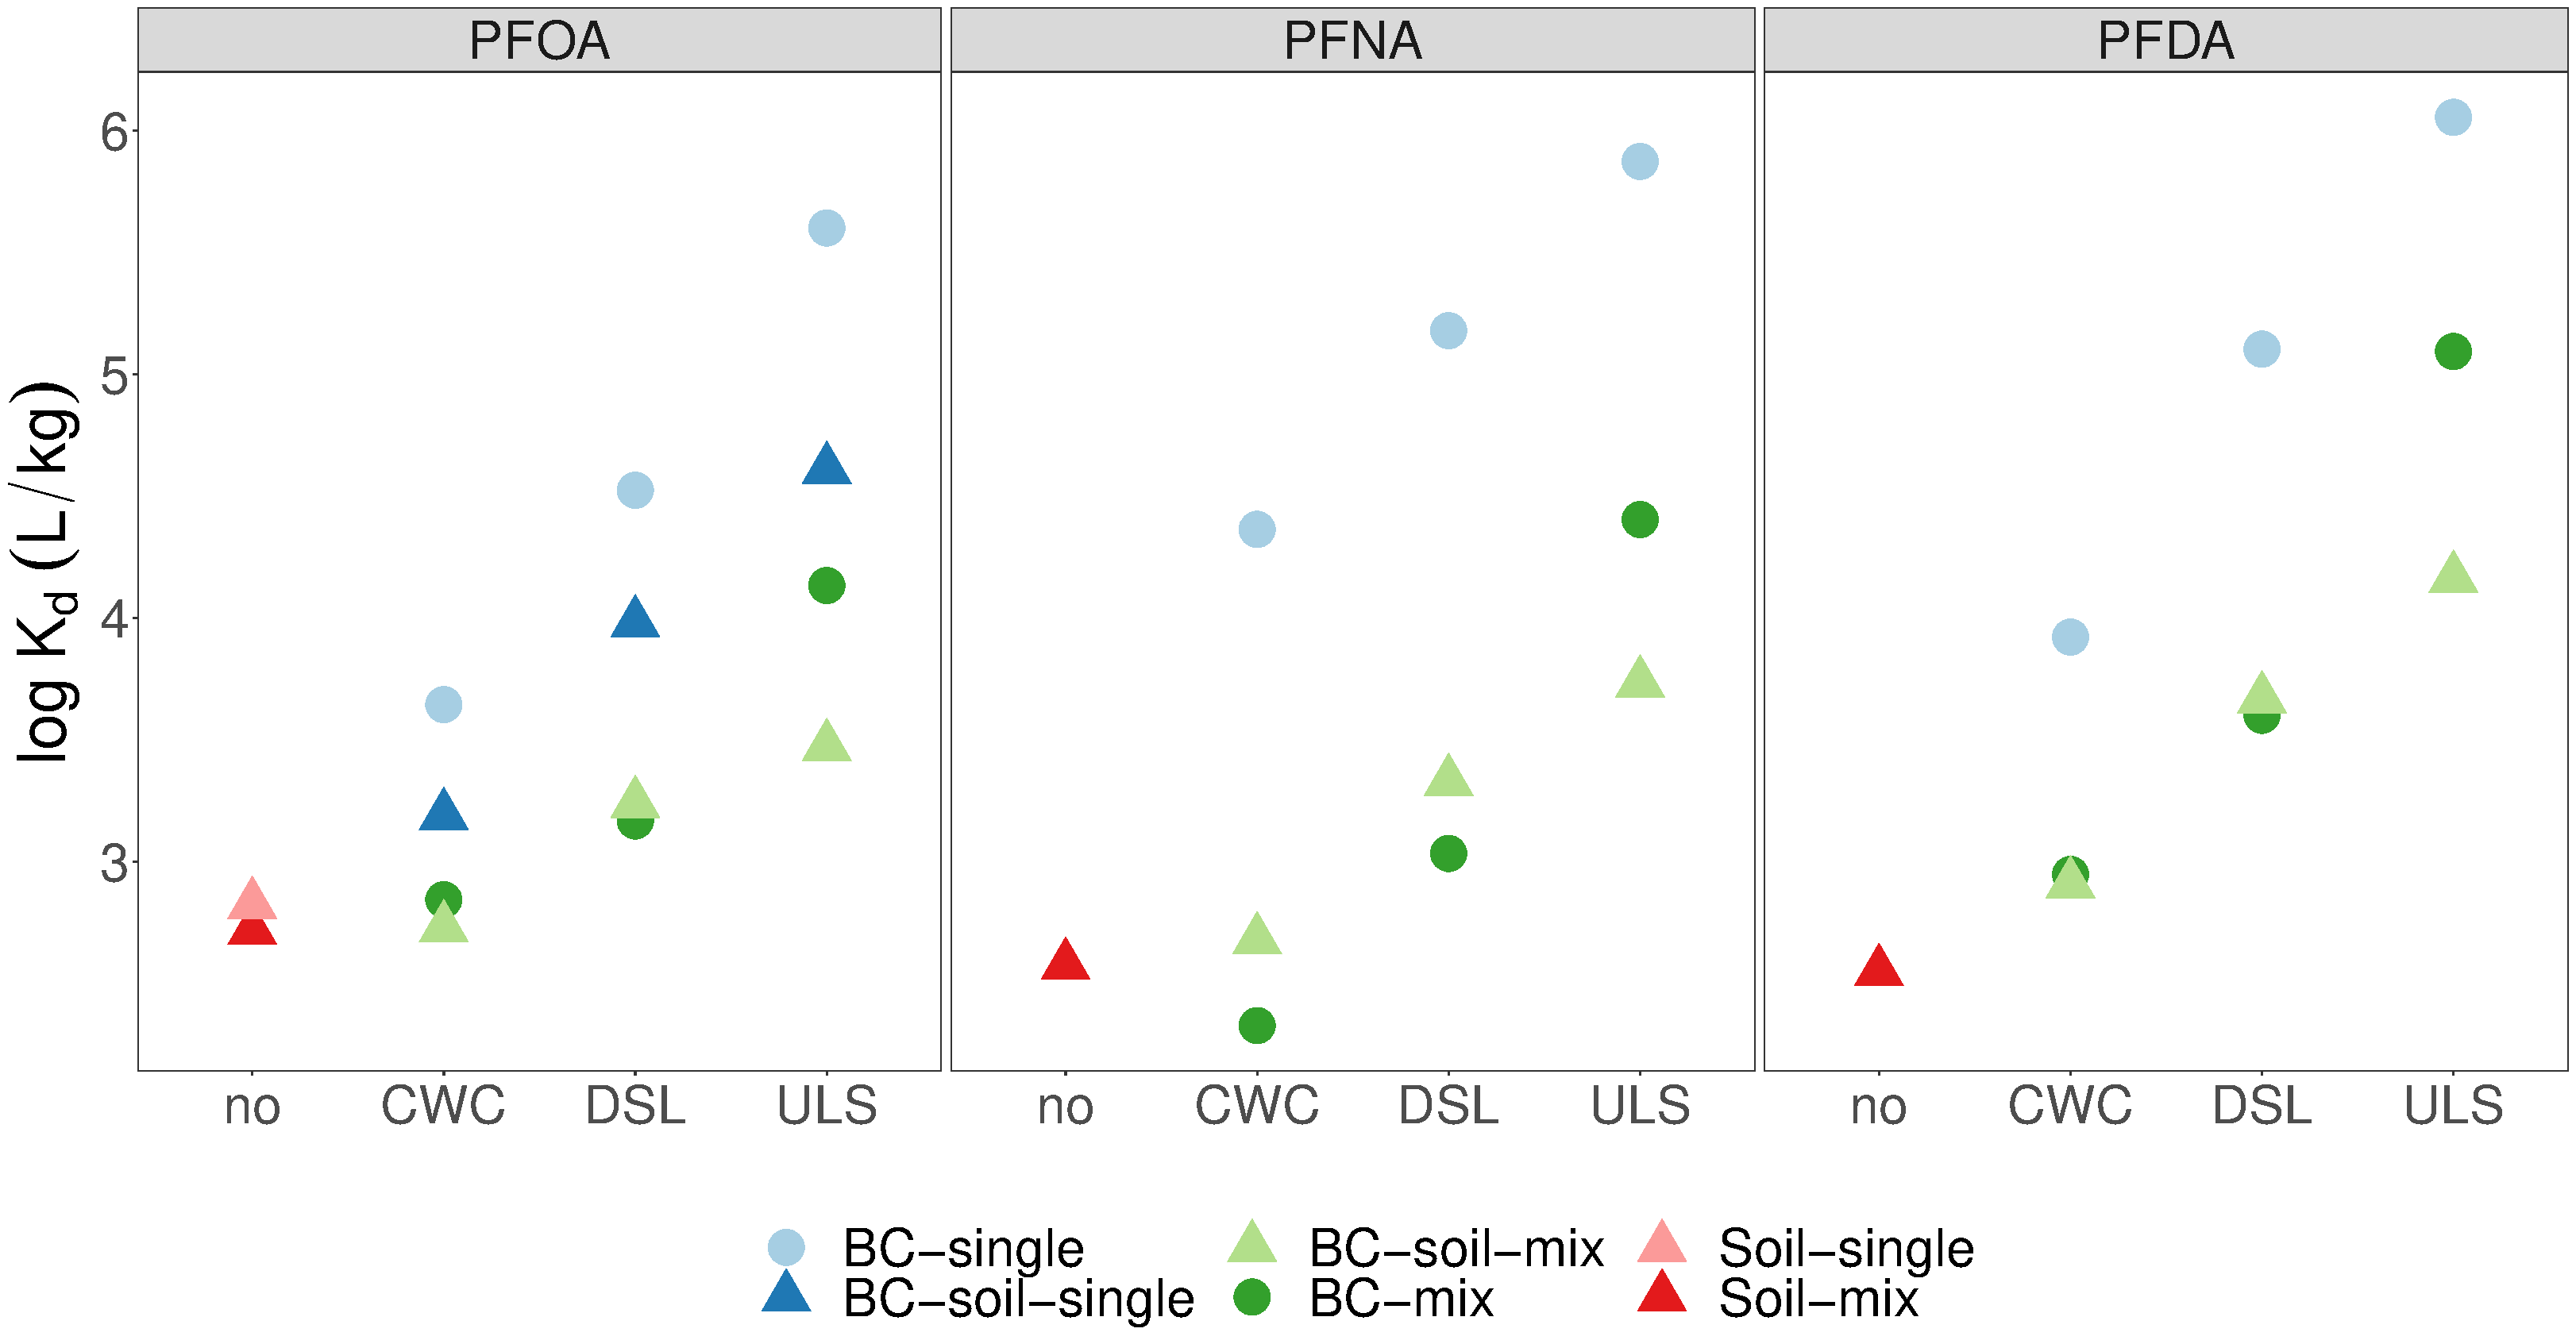
\includegraphics[width=0.75\textwidth]{R/figs/C10.pdf}
            \subcaption{Sorption capacity of each TC in single, mixed, single-soil, and mixed-soil systems spiked at SC10 (191, 330, 117, 1 953, 1 409, and 3 830 \textmu g L\textsuperscript{-1} for C5-C10, respectively) on each biochar (CWC, DSL, ULS) and soil only (no).}
            \label{subfig:C10}
        \end{subfigure}
        \begin{subfigure}[]{\linewidth}
            \centering
            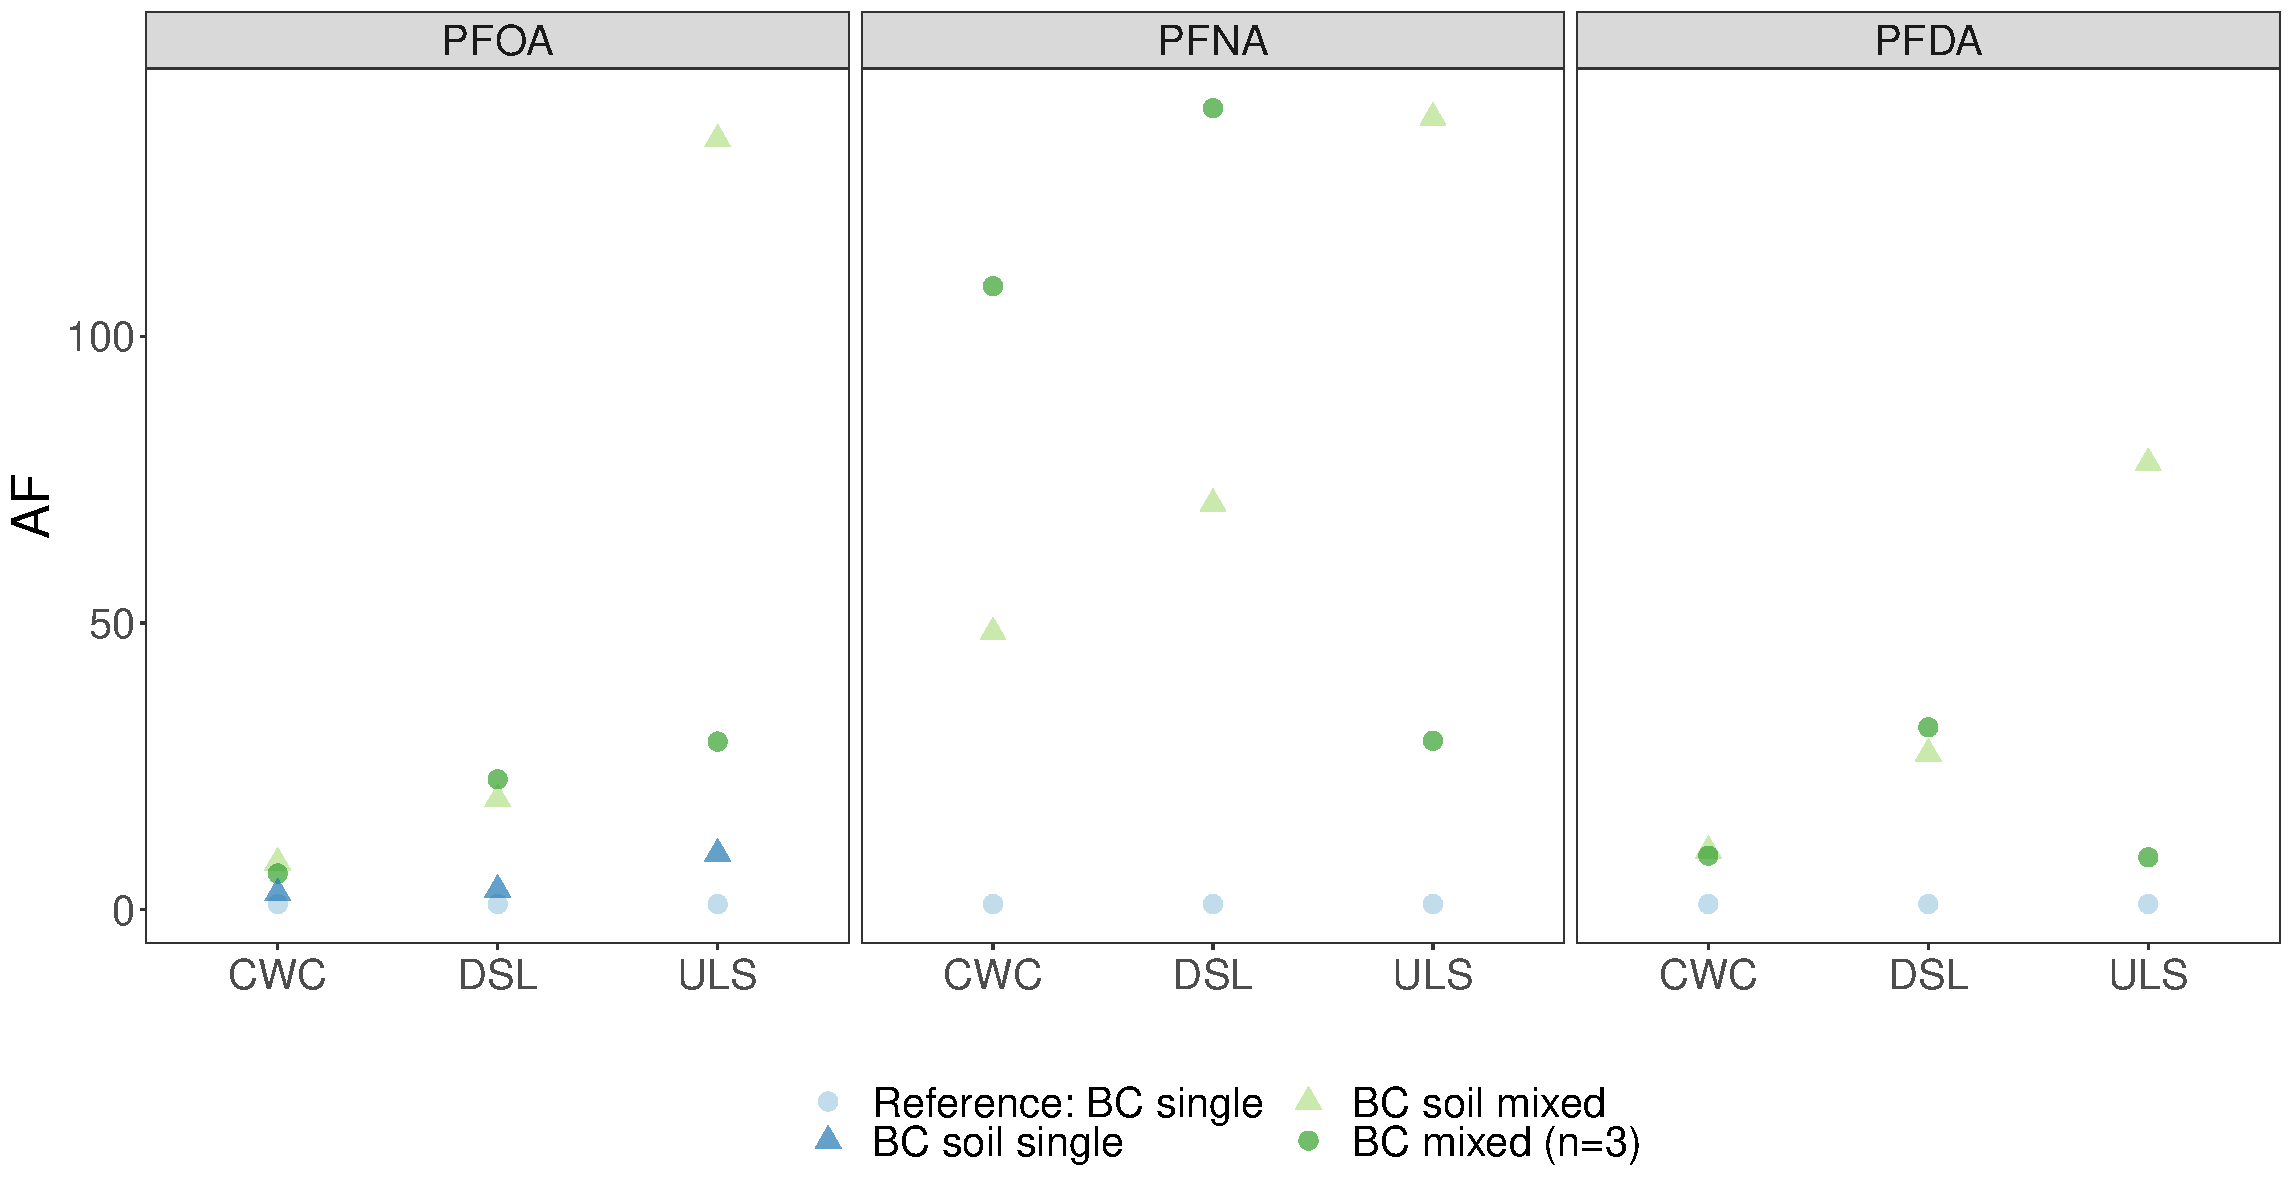
\includegraphics[width=0.75\textwidth]{R/figs/Attenuation_factors_C10_OND.pdf}
            \subcaption{Attenuation factors at C10 for C8-C10 calculated as the fraction of $K_d$ for mixed/soil/mixed and soil samples over $K_d$ of BC single (\cref{eq:AF}). BC cocktails are spiked with 7.8 mg/L total PFCA and BC soil cocktails with 10.8 mg/L (the difference is explained in the corresponding section). See \cref{tab:spikeConcentrations} for spike concentrations used for each PFCA in the single-spike and cocktail-spike batch tests.}
            \label{subfig:AF}
        \end{subfigure}  
    \caption{Reduction in \textbf{(a)} $log~K_d$ at SC10 and \textbf{(b)} attenuation factors at SC10.}
    \label{fig:C10_AF}
\end{figure}

\subsection{Sorption attenuation of PFOA isotherms}
As discussed in the previous section, the cocktail effect contributes the greatest to sorption attenuation than the presence of soil. In the PFOA-facets of \crefrange{subfig:C10}{subfig:AF}, the effect of soil on $K_d$ is visualized by the difference in the blue circles and triangles. $log~K_d$ drops by 65\%, 71\%, and 90\% for CWC, DSL and ULS, respectively. 
Attenuation is lowest for BC soil single, 12-18 \% of maximum sorption, but note that only PFOA was spiked for this batch test feedstock. Single-spikes in soil was only performed for PFOA, whose sorption is weaker than BC single, but stronger than cocktails in both BC and BC-soil. This suggests that sorption attenuation by competing congeners is higher than by the presence of soil. Applied to real-world conditions, this means that soil amended with BC is more effective in removing PFCAs at low concentrations than highly contaminated soil with a mixture of compounds and high total water concentration of PFCAs.

Parallel isotherms means that attenuation is the same across the whole concentration range, such as between BC single and BC soil single for ULS, whereas for some isotherms attenuation is minimal at low concentrations and increases with increasing spike concentration, which is the case for the DSL isotherms. That attenuation factors increases with increasing concentration is explained by the non-linear sorption at higher concentrations, so when spike concentration increases, sorption attenuation is enhanced.   

\cref{fig:PFOA_attenuation} isotherms for BC single. The isotherms are spiked with the same concentrations and shows that they have similar $C_s$ concentrations. This indicates that more PFCA in solution is needed to push the same amount of molecules onto the solid phase in presence of soil because soil has an attenuating effect by competitive sorption and pore blocking. 

Efficiency of biochar sorbents in complex systems must be evaluated in order to say something about their suitability for the intended uses because simultaneous presence of a diverse suite of organic contaminants with soil and sediment generally change sorption mechanisms and weakens sorption strength \citep{zhou2010sorption}.

\begin{figure}[htb]
    \centering
    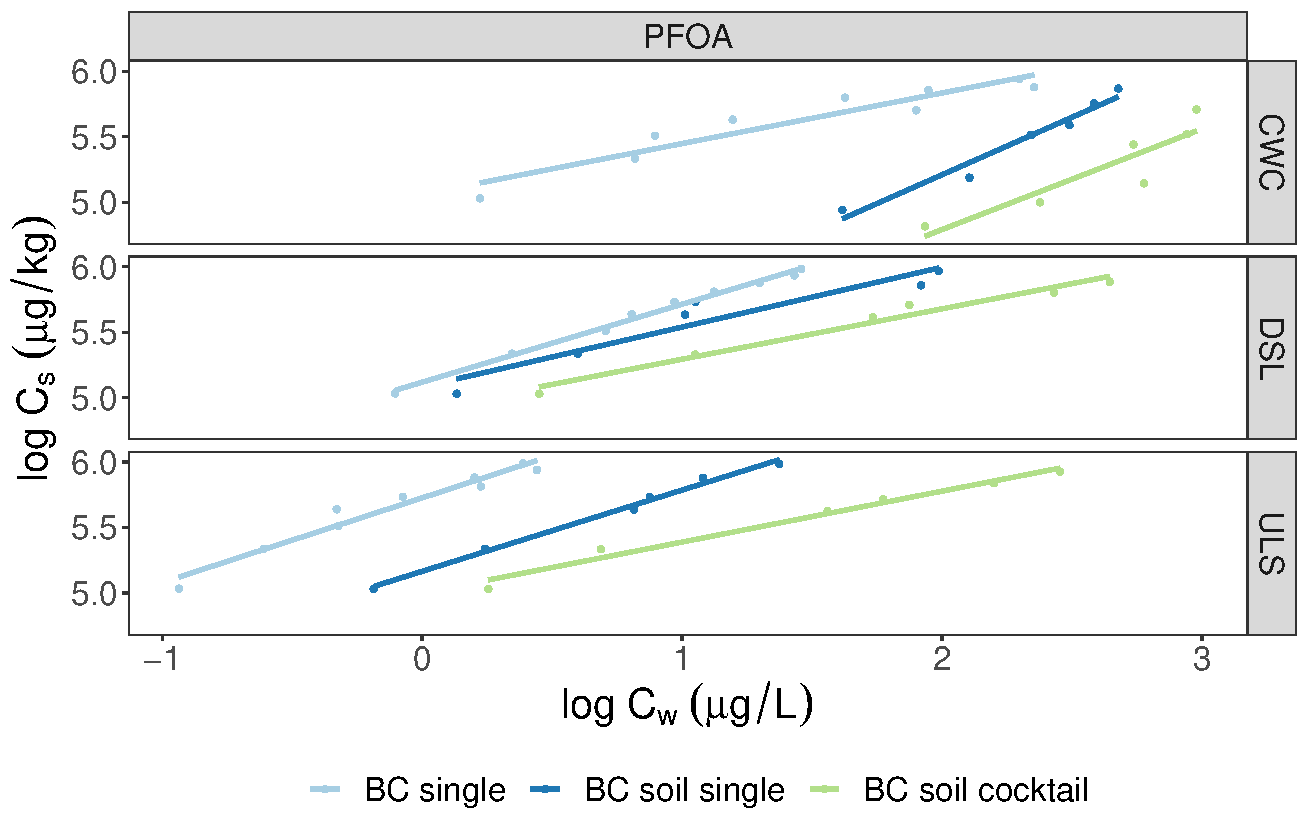
\includegraphics[width=0.8\textwidth]{R/figs/Attenuation_isotherms_PFOA.pdf}
    \caption{Sorption isotherm comparison for PFOA single-compound spike in biochar (BC single), single-compound spike in soil-biochar (BC soil single), and PFOA spiked in a cocktail in soil-biochar showing attenuation by soil and competing congeners.}
    \label{fig:PFOA_attenuation}
\end{figure}

\subsection{Sorption processes in natural systems}
Only $~7\%$ of the numerous minerals in global soils have surfaces that are net positively charged at ambient pH, most importantly Fe-oxides and Al-oxides. 
Pore filling/clogging see \citep{Li2019}
Important factors with sorbent addition:
Time: slow mass transfer under unmixed conditions for PCBs, transfer from sediment to biochar takes time \citep{Werner2006}
Fouling: weakening of sorbent sorption by natural organic matter, oil, competing contaminants

\subsection{Freundlich sorption non-linearity}\label{sec:non-linearity}
$n_F$ is a dimensionless empirical parameter that represents sorption linearity. All isotherms experience sorption site attenuation at increasing concentrations indicated by $n_F<1 $ (\cref{tab:summary_stats_single}, which is consistent with the Freundlich model and other studies where sorption to biochar sees $n$-values typically around 0.3-0.7 \citep{Cornelissen2005}. 

The concentration range acheived for each isotherm is important  ULS and DSL gave isotherms typically across 0-1.5 orders of magnitude, which indicates that either higher spike concentrations or a lower BC dosage should have been used for the batch tests and that the sludge biochars have a higher sorptive capacity compared with CWC. The batch tests were spiked at 10 concentrations over four orders of magnitude where the lowest concentration was aimed at being close to the instrumental LOQ. Poor signals were achieved for the SC1 points and were removed from the data analysis to improve the certainty of the regression analysis. By doing this the spike concentration interval was reduced to two orders of magnitude \cref{tab:spikeConcentrations}. The concentration range achieved was an average of 1.3 log units for the batch test filtrate, in contrast to the desired concentration range over 4 log units. In retrospect, spike concentrations at each log unit should have been selected instead of spreading the ten concentrations evenly across the concentration range. Gaining valid points across a wider concentration range could affect the $n_F$-value acheived.

From other studies, $K_F$ increases and $n_F$ decreases with decreasing O/C, H/C, and N/C ratios \citep{Cornelissen2005}. However, this study $K_F$ decreases with decreasing O/C, H/C, and N/C ratios, and no clear trend is seen for $n_F$. Meanwhile, it does seem like the nonlinearity coefficients for CWC are more stable with increasing chain lengths than ULS and DSL. Additionally, comparing $n$ across compound isotherms does not make sense due to different spike concentrations being used for each compound. \citep{yin2022insights} suggests that electrostatic interactions between PFCAs and sediment can contribute to further enhancement of saturation of the adsorption sites and that intermolecular electrostatic repulsion between the individual molecules could also result in nonlinear sorption \citep{higgins2006sorption,yin2022insights}.

The Freundlich coefficient of non-linearity ($n_F$), is a measure of sorption capacity within the concentration range acheived for the sorption isotherms. A lower $n_F$ indicates that sorption sites are starting to be saturated and the biochar is closer to its maximum sorption capacity. cocktail effect on non-linearity and sorption capacity: and that limiting biochar adsorption capacity at high concentrations require more PFAS present in solution to make

\citep{yin2022insights} attributes non-linear sorption to three explanations: 1) complex composition of biochar with negative, positive and neutral charges within same matrix, 2) successive saturation of adsorption sites, 3) electrostatic interactions between the PFASs and sediment, 4) electrostatic repulsion from negatively charged carboxylate groups. 

Sorption non-linearity ($n<1$) occurs due to the complex composition of sediment/biochar with both positive and negative charges contributing to either attraction or repulsion, as well as hydrophobic surfaces, and indicates successive saturation of these adsorption sites \citep{yin2022insights}.  

For the short-chain compounds (PFPeA and PFHxA), Correlations are poor which results in higher standard errors and slopes that are unrealistic (PFHxA-DSL: n=1.11 and PFHpA-ULS: 1.08). Possible explanations for the poor correlations for PFPeA and PFHxA are poor biochar affinity, but the standard error is also large so that the isotherm may actually be linear ($\pm$ 0.11 for both). For PFPeA- and PFHxA-CWC, it appears that CWC sorption sites have been saturated since most points center around the same area, which means that CWC reaches sorption maximum at $~$4 000 $\mu g~kg^{-1}$. However, four points are insufficient to conclude that CWC has the lowest affinity and capacity to sorb short-chain PFCAs. The CWC isotherms had the widest concentration intervals for $C_w$, which can be explained by CWC being the weakest sorbent of the three biochars studied, resulting in higher aqueous concentrations than for the sludge biochars. 

Freundlich non-linearity \citep{yu2009sorption}
Freundlich fitting is mostly used for sorbents with more heterogeneous surfaces, such as waste-based biochar. Factors that contribute to non-linear sorption is a sorption site heterogeneity and surface energy 

%%%%%%%%%%%%%%%%%%%%%%%%%%%%%%%%%%%%%%%%%%%%%%%%%%%%%%%%%%%%%%%%%%%%%%%%%%%%%%%%%%%%%%%%%%%%%%%%%%%%%%%%%%%%%%%%%%%%%%%%%%%%%%%%%%%%%%%%%%%%%%%%%%%%%%%%%%%%%%%%%%%%%%%%%%%%%%%%%%%%%%%%%%%%%%%%%%%%%%%%%%%%%%%%%%%%%%%%%%%%%%%%%%%%%%%%%%%%%%%%%%%%%%%%%%%%%%%%%%%%%%%%%%%%%%%%%%%%%%%%%%%%%%%%%%%%%%%%%%%%%%%%%%%%%%%%%%%%%%%%%%%%%%%%%%%%%%%%%%%%%%%%%%%%%%%%%%%%%%%%%%%%%%%%%%%%%%%%%%%%%%%%%%%%%%%%%%%%%%%%%%%%%%%%%%%%%%%%%%%%%%%%%%%%%%%%%%%%%%%%%%%%%%%%%%%%%%%%%%%%%%%%%%%%%%%%%%%%%%%%%%%%%%%%%%%%%%%%%%%%%%%%%%%%%%%%%%%%%%%%%%%%%%%%%%%%%%%%%%%%%%%%

\section{Soil properties}\label{sec:Soil}
The soil used in the batch tests was characterized as a fine sand (0.1 to 0.3 mm) with 1.3 \% TOC (pH 5.38 \textpm 0.02, CEC 2.63 \textpm 0.06 meqv 100 g\textsuperscript{-1}). Total element concentrations and exchangeable ion concentrations are in \cref{appSec:elements}, \cref{apptab:soil}. Soil extraction showed no native target analytes present. 

Upon filtration, each batch test category was different in its ease of filtration due to various degree of suspended particles, which also resulted in different filtrate color \cref{subfig:filtrate}. The soil batch tests with ULS and DSL were more transparent than soil only and soil-DSL, which is attributed to complexation of inorganic species present in the sludge chars. Since filters were clogged and had to be exchanged up to three times during filtration, both clogging resulting in reduced filter pore size and multiple filter exchange are possible sources of errors for the measurement of accurate $C_w$. Filter blanks were only conducted for BC-water samples and showed no significant effect (see \cref{subsec:FB}, but filtration with soil may be different. 

As described in \cref{sec:S-BC}, the batch tests with soil and soil-CWC Aggregation of humic substances as brown fluff was observed upon addition of 1 M acetic acid to pH 3 pre-SPE for the most colored filtrated samples \cref{subfig:precip}, indicative of humic acids. At low pH, humic acids protonate, which leads to less electrostatic repulsion between acid functional groups within the DOC molecules so that they aggregate and precipitate from solution. During SPE, PFCAs that had sorbed to the DOC would be extracted and contribute to an overestimation of $C_w$. 

In summary, the results and observations from the BC soil batch tests indicate that 1) waste-based biochar reduces DOC, and 2) DOC in the filtrate has potentially contributed to an overestimation of $C_w$, and hence, underestimation of $K_d$. The effect of 2) cannot be traced with the data produced and remains unsolved. 

\begin{figure}[tbh]
\subfloat[\label{subfig:filtrate}]{%
  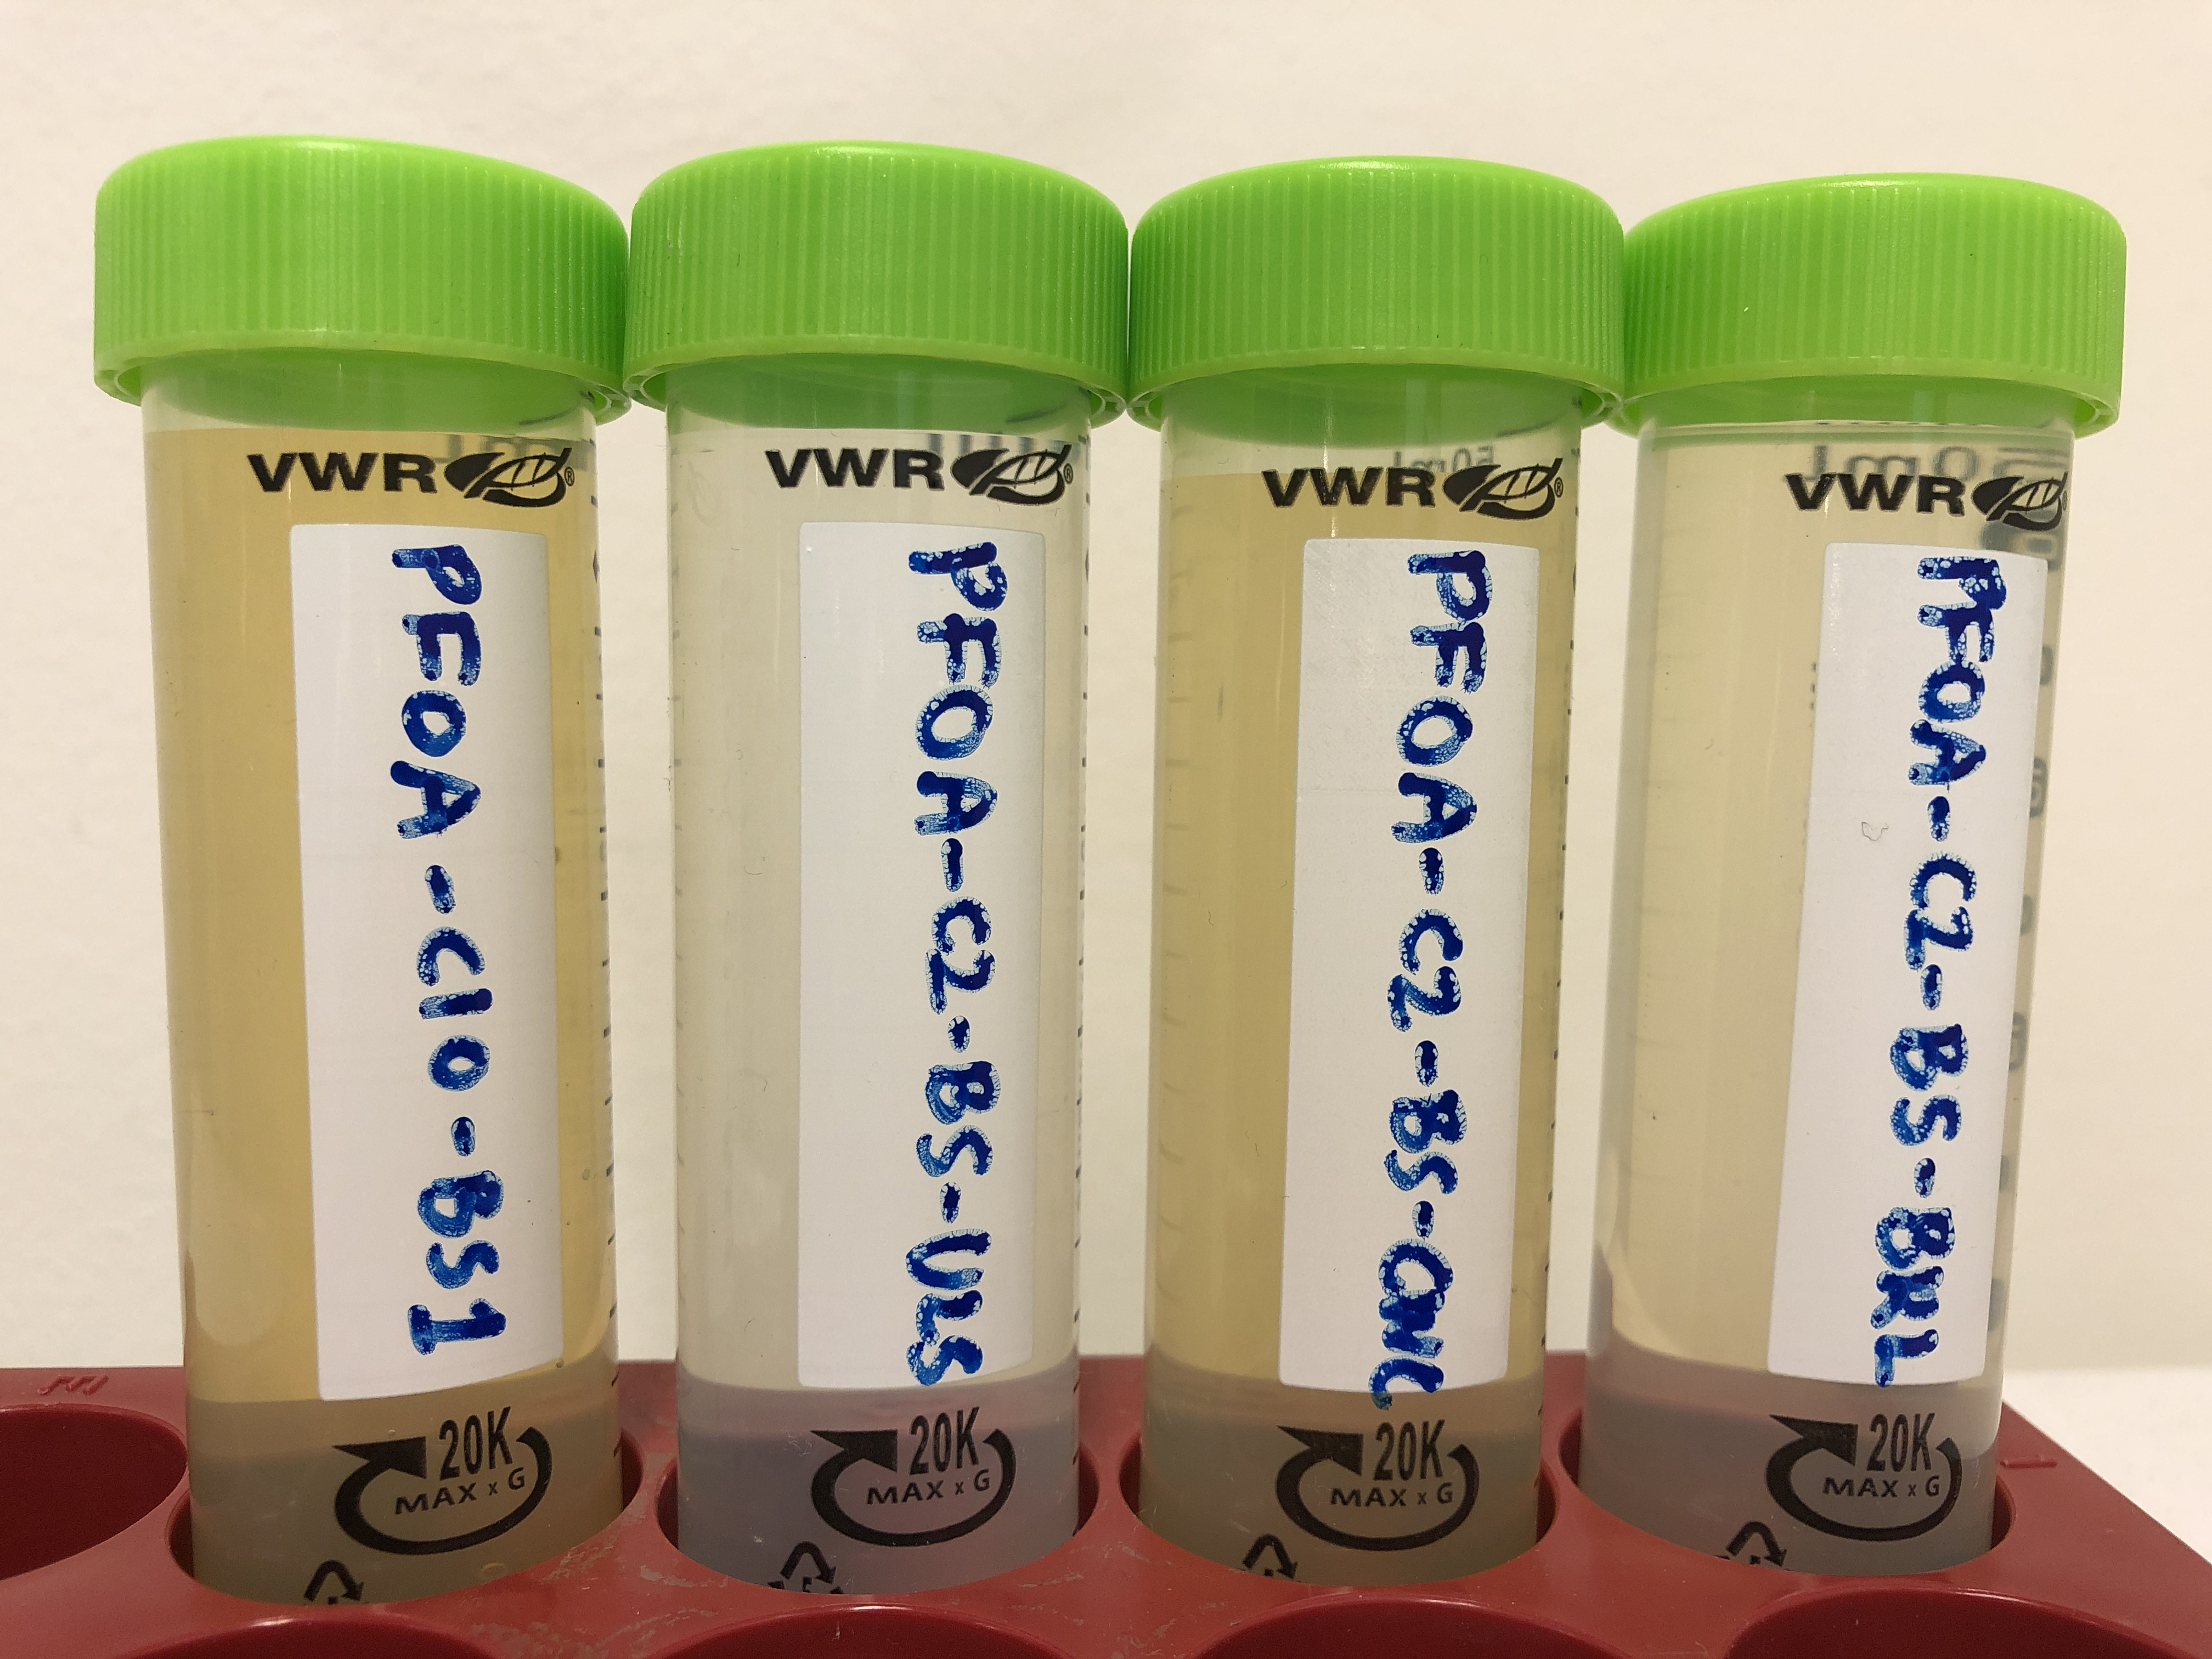
\includegraphics[width=0.45\textwidth]{Bilder/Samples/Filtrate_DOC.JPG}
}
\hfill
\subfloat[\label{subfig:precip}]{%
  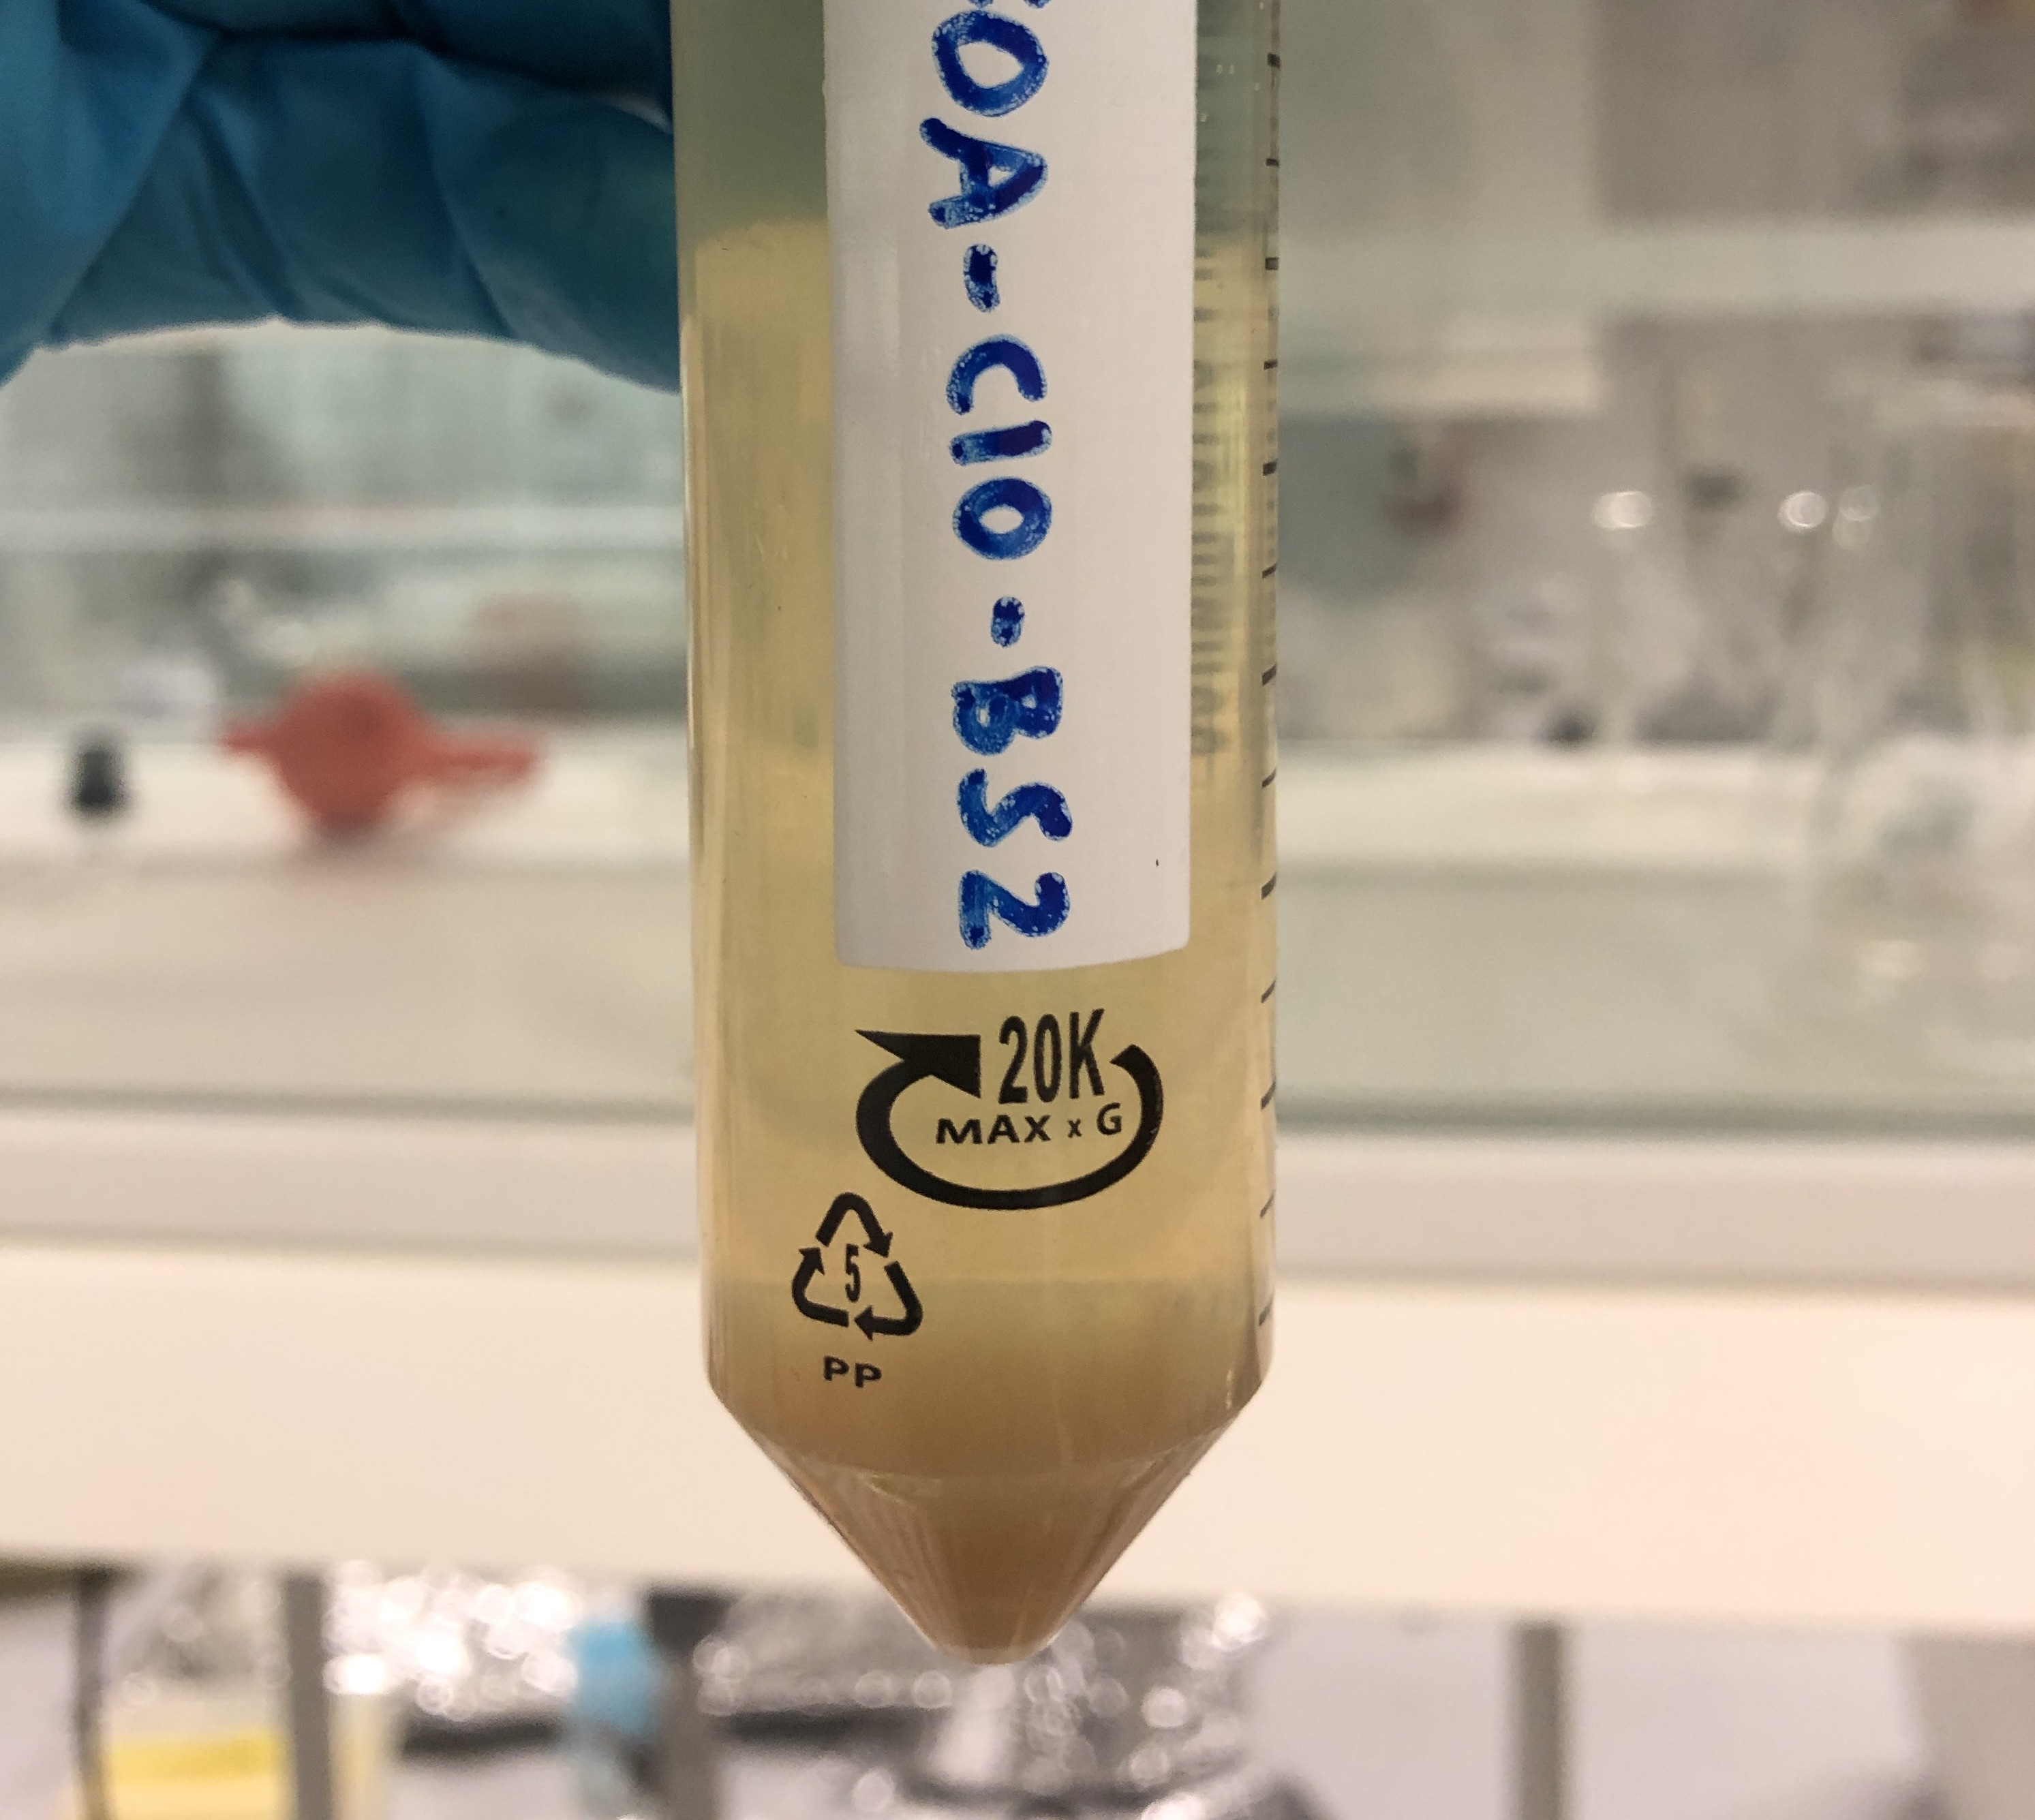
\includegraphics[width=0.38\textwidth]{Bilder/Samples/Precipitation.JPG}
}
\caption{(a) Color of filtrate for each biochar batch test. From left to right: soil only, soil+ULS, soil+CWC, and soil+DSL (BRL = DSL). (b) Precipitation observed when filtered soil samples were adjusted to pH 3 with 1 M acetic acid.}
\label{fig:DOC_tubes}
\end{figure}


%%%%%%%%%%%%%%%%%%%%%%%%%%%%%%%%%%%%%%%%%%%%%%%%%%%%%%%%%%%%%%%%%%%%%%%%%%%%%%%%%%%%%%%%%%%%%%%%%%%%%%%%%%%%%%%%%%%%%
%%%%%%%%%%%%%%%%%%%%%%%%%%%%%%%%%%%%%%%%%%%%%%%%%%%%%%%%%%%%%%%%%%%%%%%%%%%%%%%%%%%%%%%%%%%%%%%%%%%%%%%%%%%%%%%%%%%%%
%%%%%%%%%%%%%%%%%%%%%%%%%%%%%%%%%%%%%%%%%%%%%%%%%%%%%%%%%%%%%%%%%%%%%%%%%%%%%%%%%%%%%%%%%%%%%%%%%%%%%%%%%%%%%%%%%%%%%

\section{Potential for commercializing sludge chars as sorbents}
Potential challenges with application of sewage sludge-based sorbents: leaching of heavy metals, sorption capacity, pH (although liming raises pH which is not good for sorption, addition of Ca\textsuperscript{2+} creates divalent bridging effect and complexation of PFAS molecules that enhance sorption. 

Removal efficiency, good enough for application?

Leaching of heavy metals results at PT 700 C
    As, Cd, Co, Zn, Pb for all chars Below EBC limits, Cr and Ni between lower and upper limit
    EBC = European Biochar Certificate
    Cu above EBC limits for ULS and DSL
    Enrichment factors heavy metals (?)

\subsubsection{Field conditions representativeness}

Equilibrium conditions vs laboratory batch tests
BC dose

Are the results representative of what goes on in real life? Sorption by shaking for 14 days represent an assumed equilibrium between PFCAs in the water and soil phase. A comparable situation in the field would be washing of the soil with large amounts of water such as during heavy rainfall. This will only be the case during occasional stormwater events and thus the results from this research could benefit from being supplemented with results from leaching tests using biochar mixed with soil. However, the relationship:

\begin{align}
    \frac{k_1}{k_2}
\end{align}

where \(k_1\) is the PFCA sorption (adsorption and absorption) rate and \(k_2\) is the PFCA desorption rate, where \(k_1>>k_2\), which indicates that sorption is many times higher, and in an equilibrium situation, sorption and desorption will be at steady state \citep{Cornelissen2005}. 

\section{Sustainability}\label{sec:LCA}
\subsection{Life cycle impact assessment (LCIA)}
LCA (life cycle assessment), sustainability aspects of production of biochar
High operating energy and cost different technologies \citep{Alhashimi2017}
Energy demand pyrolysis 
Energy production occurs from pyrolysis reactions through the gaseous and liquid fuels that are created as co-products, however, bio-oil from pyrolysis of sewage sludge is likely unsuitable as energy source
Describe pyrolysis process for AC
"compared to the highly exothermic incineration, most of the pyrolytic reactions are endothermic consuming energy of around 100 kJ kg\textsuperscript{-1}
pyrolysis: generally characterized based on heating rate, temperature and gas residence time (slow pyrolysis to fast pyrolysis)
sludge gasification: converts dried WAS into combustible gases (syngas) under partial oxidation at elevated temperatures of 700-1000 \textdegree C
Will pyrolysis remove PFAS? Draw parallel to pyrolysis of PTFE (Teflon) that occurs when pan is heated to above 300 \textdegree C, can get polymer fume fever from toxic fumes (carbonyl fluoride and trifluoroacetyl fluoride) 
What matter will the use of biochar be in the green shift? LCA, circular economy

If CWC was activated, it would likely become a much better sorbent because most of the smallest pore spaces previous inaccessible to PFAS would be expanded, giving CWC the lowest log SA/PV/C ratio. 

\subsection{The Charcoal Vision}
\citep{Laird2008}: "A win-win-win scenario for simultaneously producing bio-energy, permanently sequestering carbon, while improving soil and water quality". l, 

\subsection{The 4 per mille initiative}
The 4 per 1000 initiative United Nations climate Change conference of December 2015 (COP21)\footnote{\url{https://www.4p1000.org/}}. Annual growth rate of 0.4 \% in the soil carbon stocks, or 4 \textperthousand  per year in the first 30-40 cm of soil a means to reach the goals set forward by the Paris agreement, complement what is necessary efforts to reduce GHG emissions globally. Carbon sequestration. Goal to scale biochar for global agricultural and remediation markets. 

\subsection{Sustainable Development Goals}
Sustainable Development Goals (SDGs)

\subsection{International Biochar Initiative}
Biochar standards

\subsection{The European Green Deal}\label{sec:greendeal}
Fresh air, clean water, healthy soil and biodiversity
like ZeroPM\footnote{https://zeropm.eu}, EarthResQe\footnote{https://www.nmbu.no/en/services/centers/earthresque}, SLUDGEEFFECT\footnote{https://www.ngi.no/eng/Projects/SLUDGEFFECT}, PERFORCE\footnote{https://perforce3-itn.eu} VOW\footnote{https://www.ngi.no/eng/Projects/VOW-Valorization-of-Organic-Waste} among others  set to contribute to achieve the European Green Deal  Fresh air, clean water, healthy soil and biodiversity
14 July 2021 biochar is a means to achieve the goal to make Europe the first climate neutral continent by economic means: biochar is a potential commercial product\footnote{\url{https://ec.europa.eu/info/strategy/priorities-2019-2024/european-green-deal/delivering-european-green-deal_en}}. . 

\section{Quality control of laboratory analysis and uncertainty}
Standard concentration (but at least leads to underestimation of results)
\subsection{Spiking standard concentrations}
SPE and directly, why?

The pipettes used for making the PFCA dilutions were calibrated. The three pipettes were: 1) 2-10 mL, 2) 200-1000 \textmu L, and 3) 5-50 \textmu L. All pipettes were below the permitted coefficient of variation (CV = 0.3, 0.5, and 2 $\%$ respectively (\cref{appSec:misclab}, \crefrange{appTab:pip2-10}{appTab:pip5-50}).

Since the diameter of the centrifuge tube (30 mm) was larger than that of a volumetric flask and biochar was added prior to the dilution process, the final concentration of the sorbent-sorbate mixture may have a heightened inaccuracy. However, the volume of which 0.1 g biochar occupies can be considered insignificant due to the high absorptive capacity of biochar and small mass used. Therefore a set of 10 centrifuge tubes filled to 50 mL containing 0.1 g CWC were weighed to control the uncertainty of the final dilutions. The results from weighing show that the weight of 10 trials were not accurate but precise, which means that all samples were prepared with the same final volume even though this volume deviates from 50 mL (\cref{appTab:PPcentrifuge}). 

Volume 50 mL weighed vs by eye measurement, diameter of test tube and error
preparation of cocktail standard, not consistent, some individual pipetting. 

\subsubsection{Filter blanks no significant difference}\label{subsec:FB}

\subsection{PFAS losses during laboratory analysis}
SPE protocol, many steps, many PP test tubes transfers, saturated PFAS-solutions, internal standard (dilutions had to disregard IS because too low concentration)

\citep{Lath2019labsorb}: 
Syringe filters: sorption of PFOA to centrifuge tubes and filter membranes. Sorption onto syringe surface: negligible due to short residence time (\textless 10 s). 74\% recovery from regenerated cellulose syringe filter. No improvement in recovery was seen when conditioning the syringe filters with phosphate solution or methanol. No trend between losses of PFOA on syringe filter and increasing spike concentrations. Centrifugation only is therefore advised if possible to avoid filtration losses. 

Test tubes: Greater recoveries from glass tubes than plastic, PP poorest recovery (55-68 \% recovery)... Contact time of PFAS residing in tubes for longer than 7 days should not be of significance, as \citep{Lath2019labsorb} propose that sorption and saturation of tube walls occur within hours. 74-81 \% recovery for PP when testing dependence on pH and ionic strength. Slight pH dependence, higher recovery at higher pH due to repulsion of negatively charged functional groups (PP has negative surface charge above pH 3.5-4. Bridging effect will be observed at higher pH's between cations like Ca2+, but is still considered negligible compared to the losses due to the physicochemical properties of the materials themselves. In general PP and plastics consists of mainly carbon hydrogen chains and are more hydrophobic than glassware. Sorption to tube walls saturate, so recoveries increase significantly with higher spike concentrations (e.g. for PP, 12-415 ug/L spiked PFOA increased recovery from 53.7-85.5 \%). Therefore, quantification of low concentrations may be subject to highest error, and in most cases will be an underestimation of dissolved concentrations. 

Use of PP test tubes, study
Higher probability of underestimating Cw for low-concentration samples because tube walls saturate – maximum number of sorption sites, there is a sorption maximum (Langmuir)

\subsection{Uncertainty}
Each of the many steps involved in the determination of the aqueous equilibrium concentrations of the target compounds will have an impact on the overall uncertainty of the results. This uncertainty starts with the preparation of PFAS standards used for spiking, pipetting of standards into each batch tests, whereby up to three pipettings were conducted per sample, weighing of sorbent dose, water volume, contamination during sample preparation and storage, filtering of samples and co-sorption onto filters and tube walls, chemical analysis by solid phase extraction and LC-MS/MS, a combination of automatic and manual peak integration, and data treatment. Therefore, it is difficult to determine the absolute uncertainty of all steps in the process, but based on previously reported estimates of uncertainty on similar work, 20-30\% uncertainty is to be expected. Details on the expected main sources of uncertainty will follow.

\subsubsection{Batch tests}
Vel, du kan jo prøve å legge sammen alle de feilene. Det finnes jo forskjellige typer feilkilder i et stort forsøksoppsett. Det man ofte ser er at det er en eller to feil som er så store at de overskygger de andre. Da er det ikke noen vits å ta med alle de små. Feilen som ofte er størst er reproduserbarhet av metoden. Altså forskjellen mellom for eksempel prøver laget i triplikater. Det du kan gjøre i oppgaven din er jo å kort diskutere feilkildene du har og identifisere de største og viktigste.

\subsubsection{Analytical}
Calibration curves and matrix effect, 3-point curve
LC-MS/MS

\subsubsection{Peak integrations}
Manual review of peak integrations
decisions to remove C1 at low signal
where observed similar peak integrations across concentrations, suspected saturation of detector, dilution of these samples